%%%%%% TEX FILE AUTOMAGICALLY PRODUCED BY  producetable.py %%%%%%
\subsection{ttH 125}
\begin{longtable}{|c|c|}
\caption{Fit Results}
\endfirsthead
\caption{Fit Results (continue)}
\endhead
\hline
\parbox{0.47\textwidth}{
\centering
{\bfseries fit-mh-125-ttH-cat0.pdf}
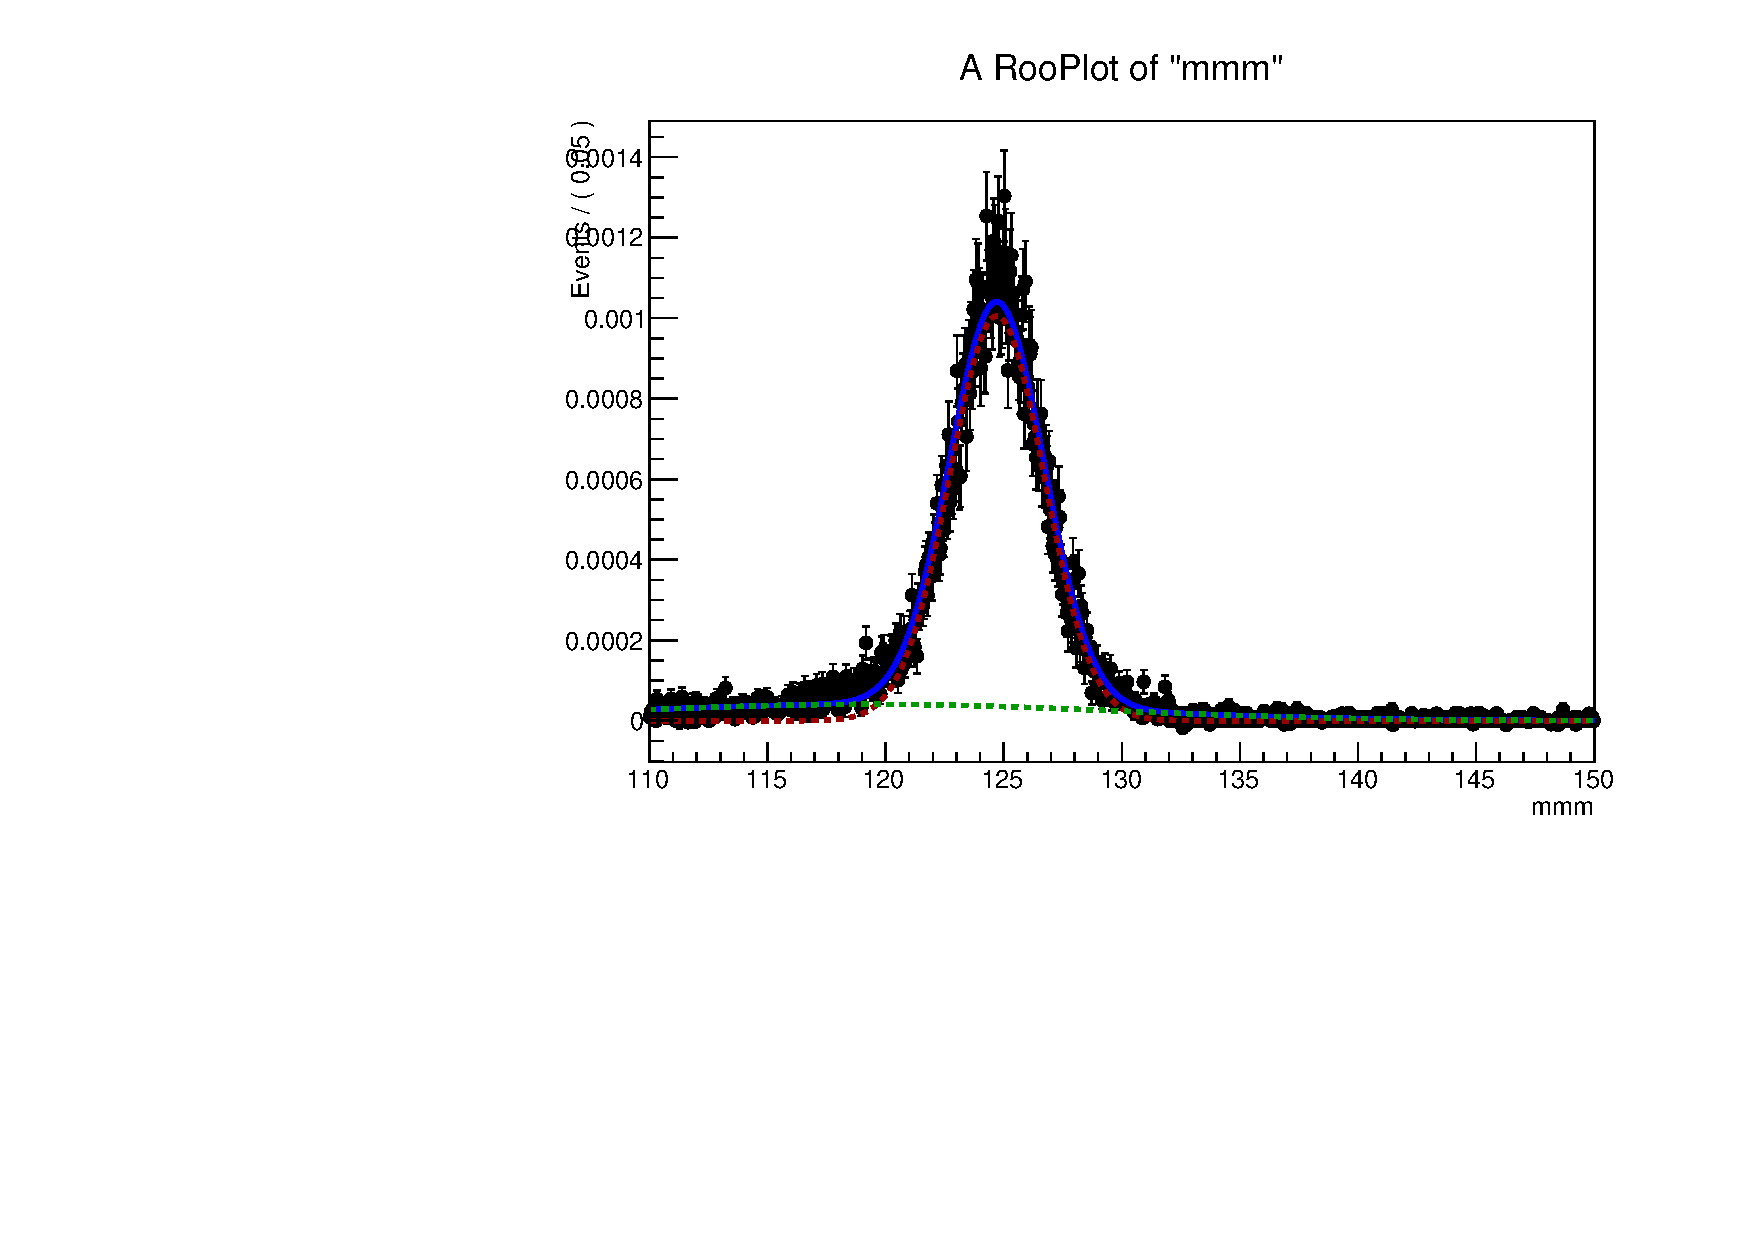
\includegraphics[width=.47\textwidth]{figures/signal_model/AppendixBdt/ttH/125/fit_mh_125_ttH_cat0.pdf}
}
 & \parbox{0.47\textwidth}{
\centering
{\bfseries fit-mh-125-ttH-cat1.pdf}
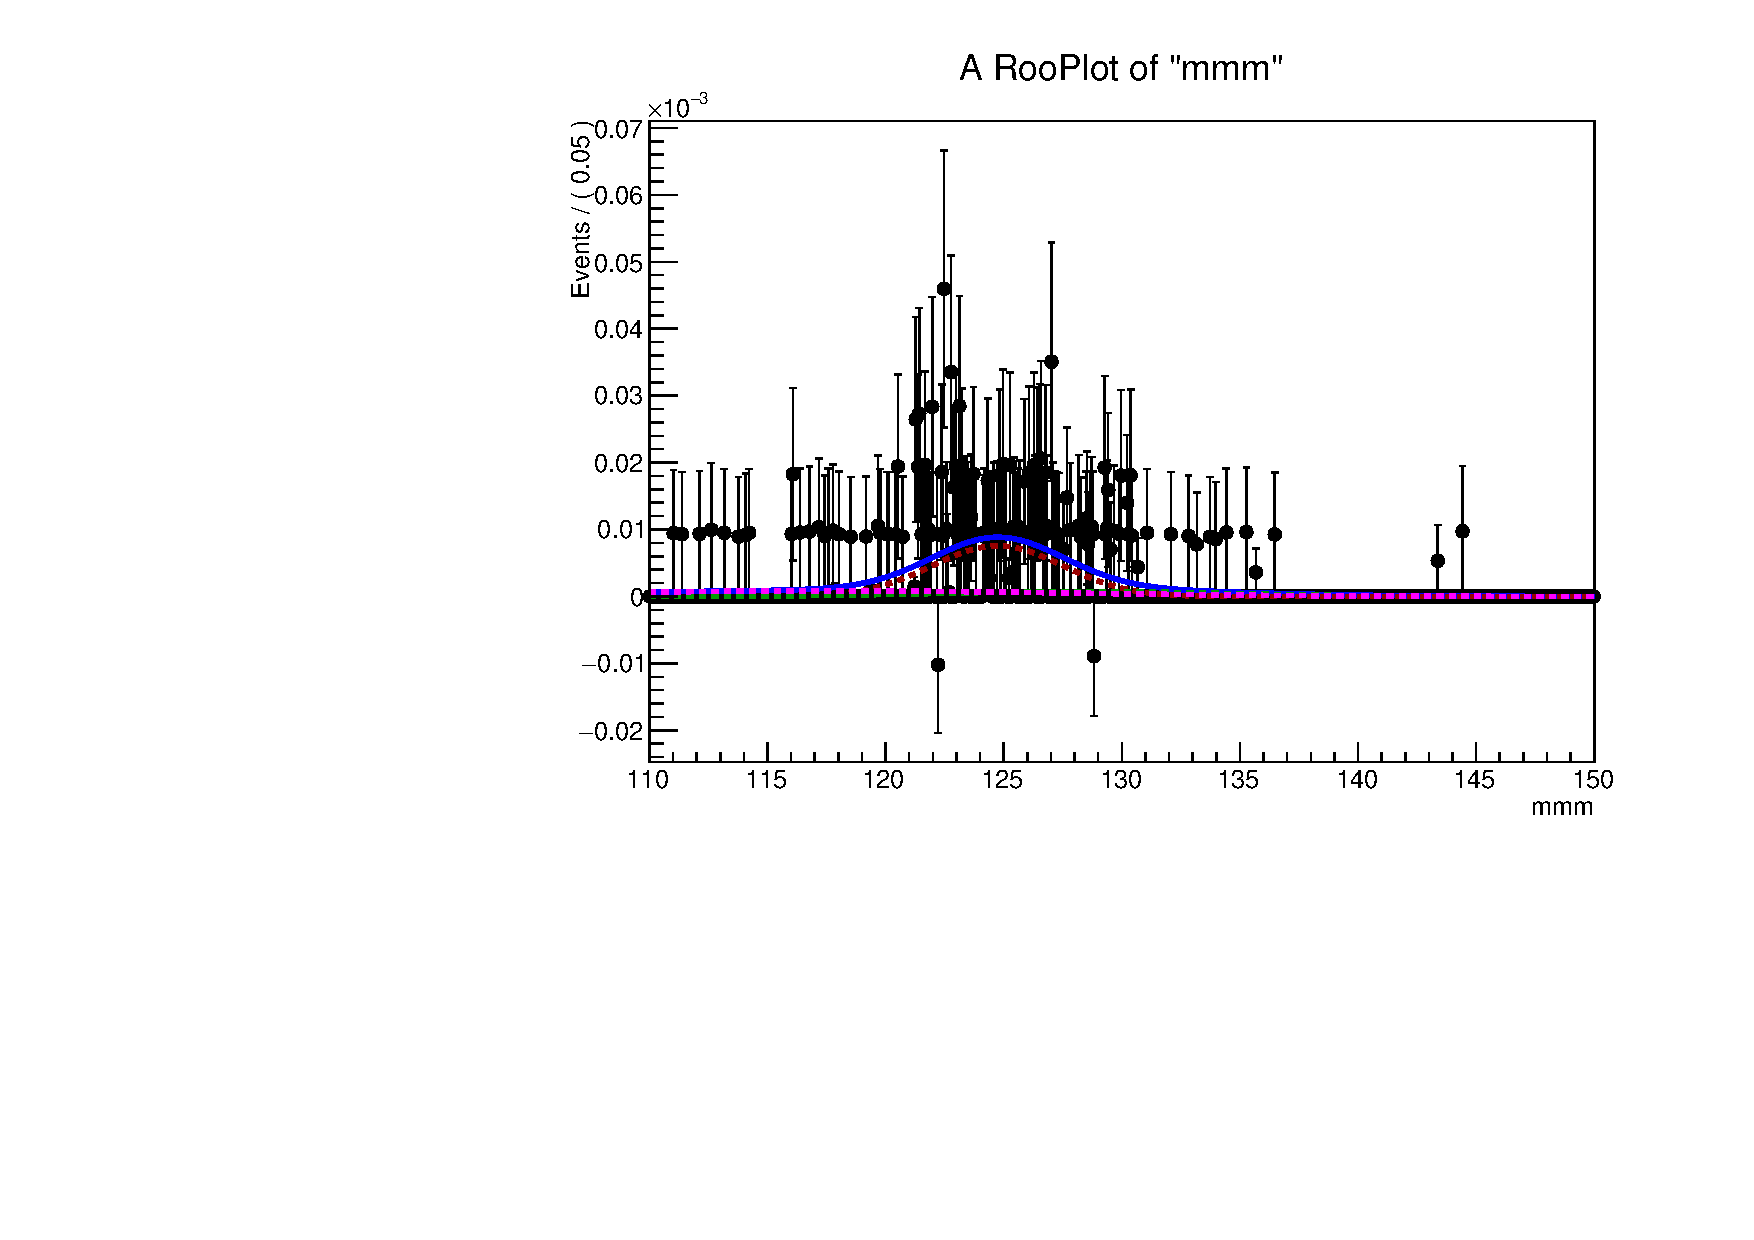
\includegraphics[width=.47\textwidth]{figures/signal_model/AppendixBdt/ttH/125/fit_mh_125_ttH_cat1.pdf}
}
 \\
\hline
\parbox{0.47\textwidth}{
\centering
{\bfseries fit-mh-125-ttH-cat2.pdf}
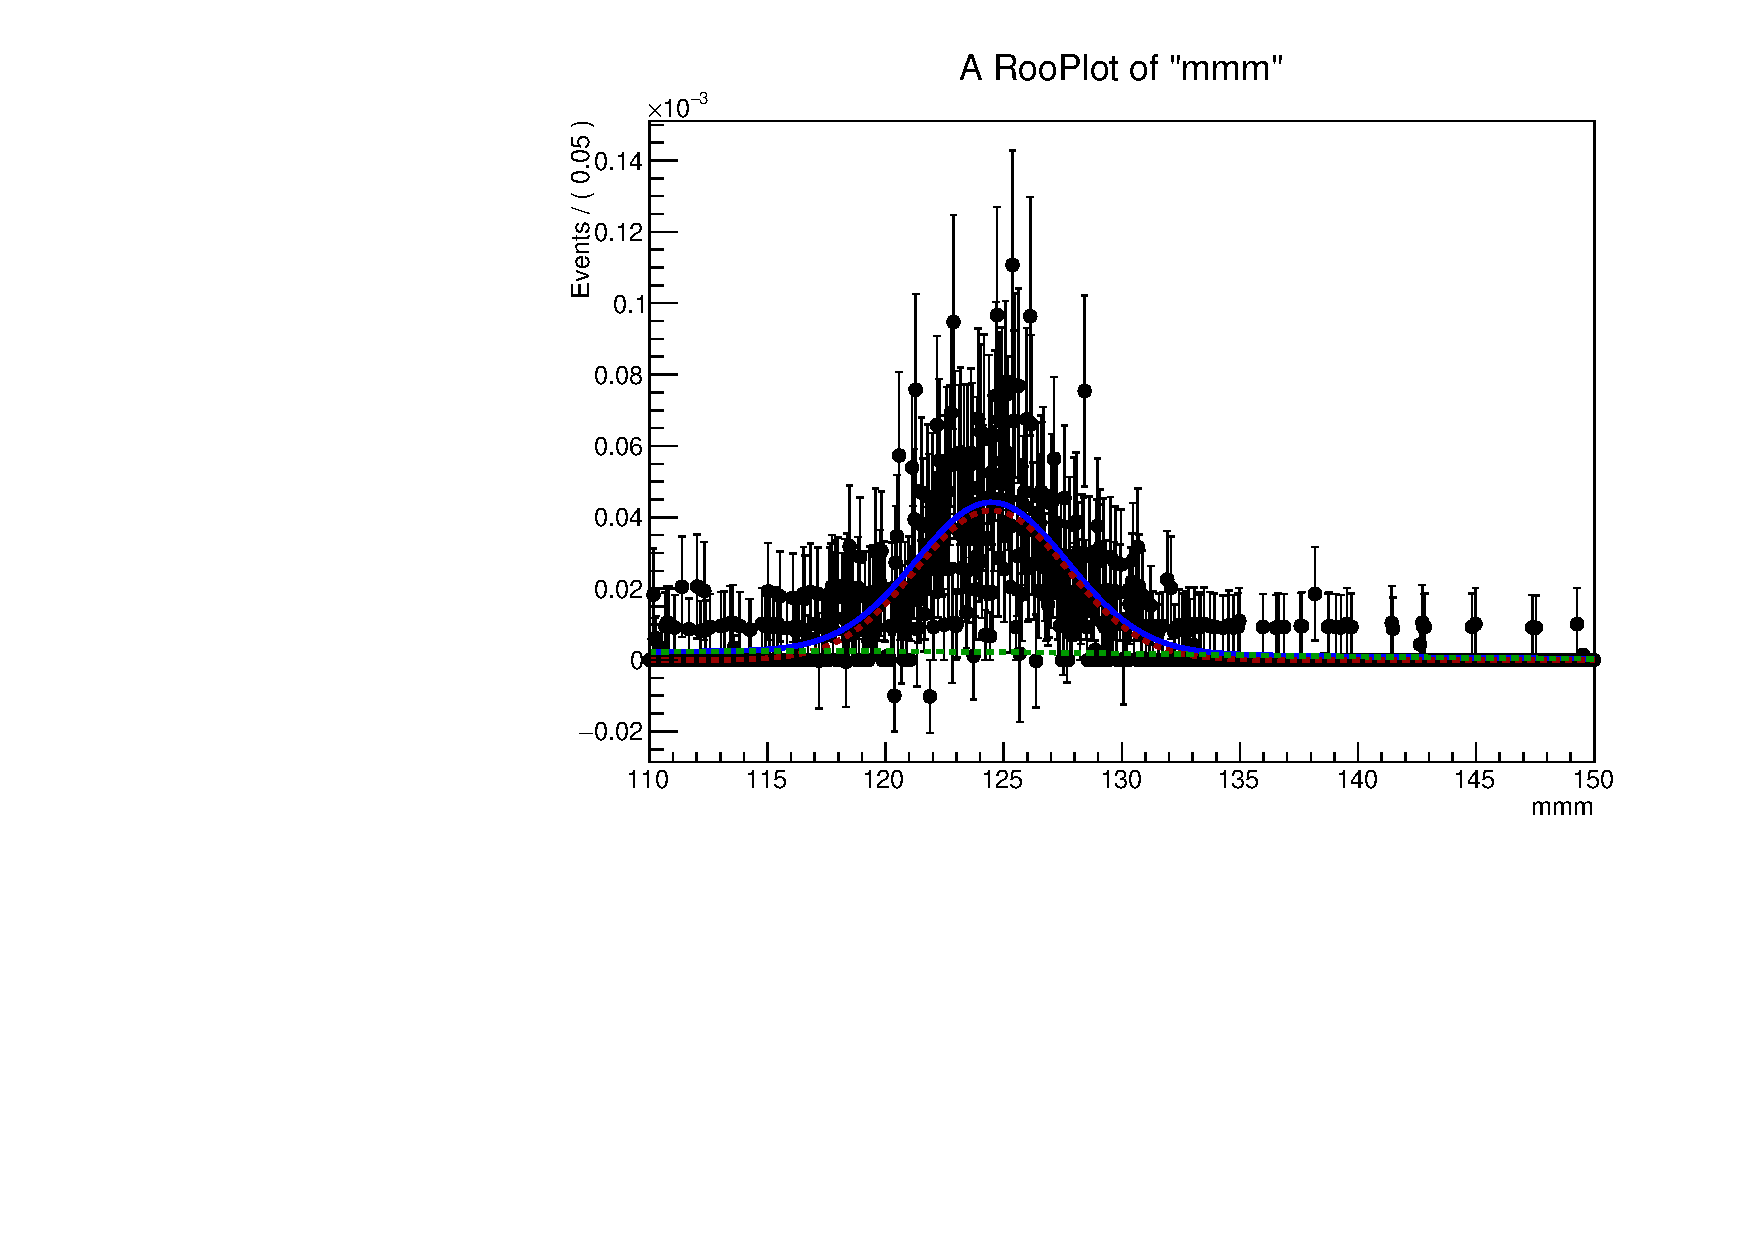
\includegraphics[width=.47\textwidth]{figures/signal_model/AppendixBdt/ttH/125/fit_mh_125_ttH_cat2.pdf}
}
 & \parbox{0.47\textwidth}{
\centering
{\bfseries fit-mh-125-ttH-cat3.pdf}
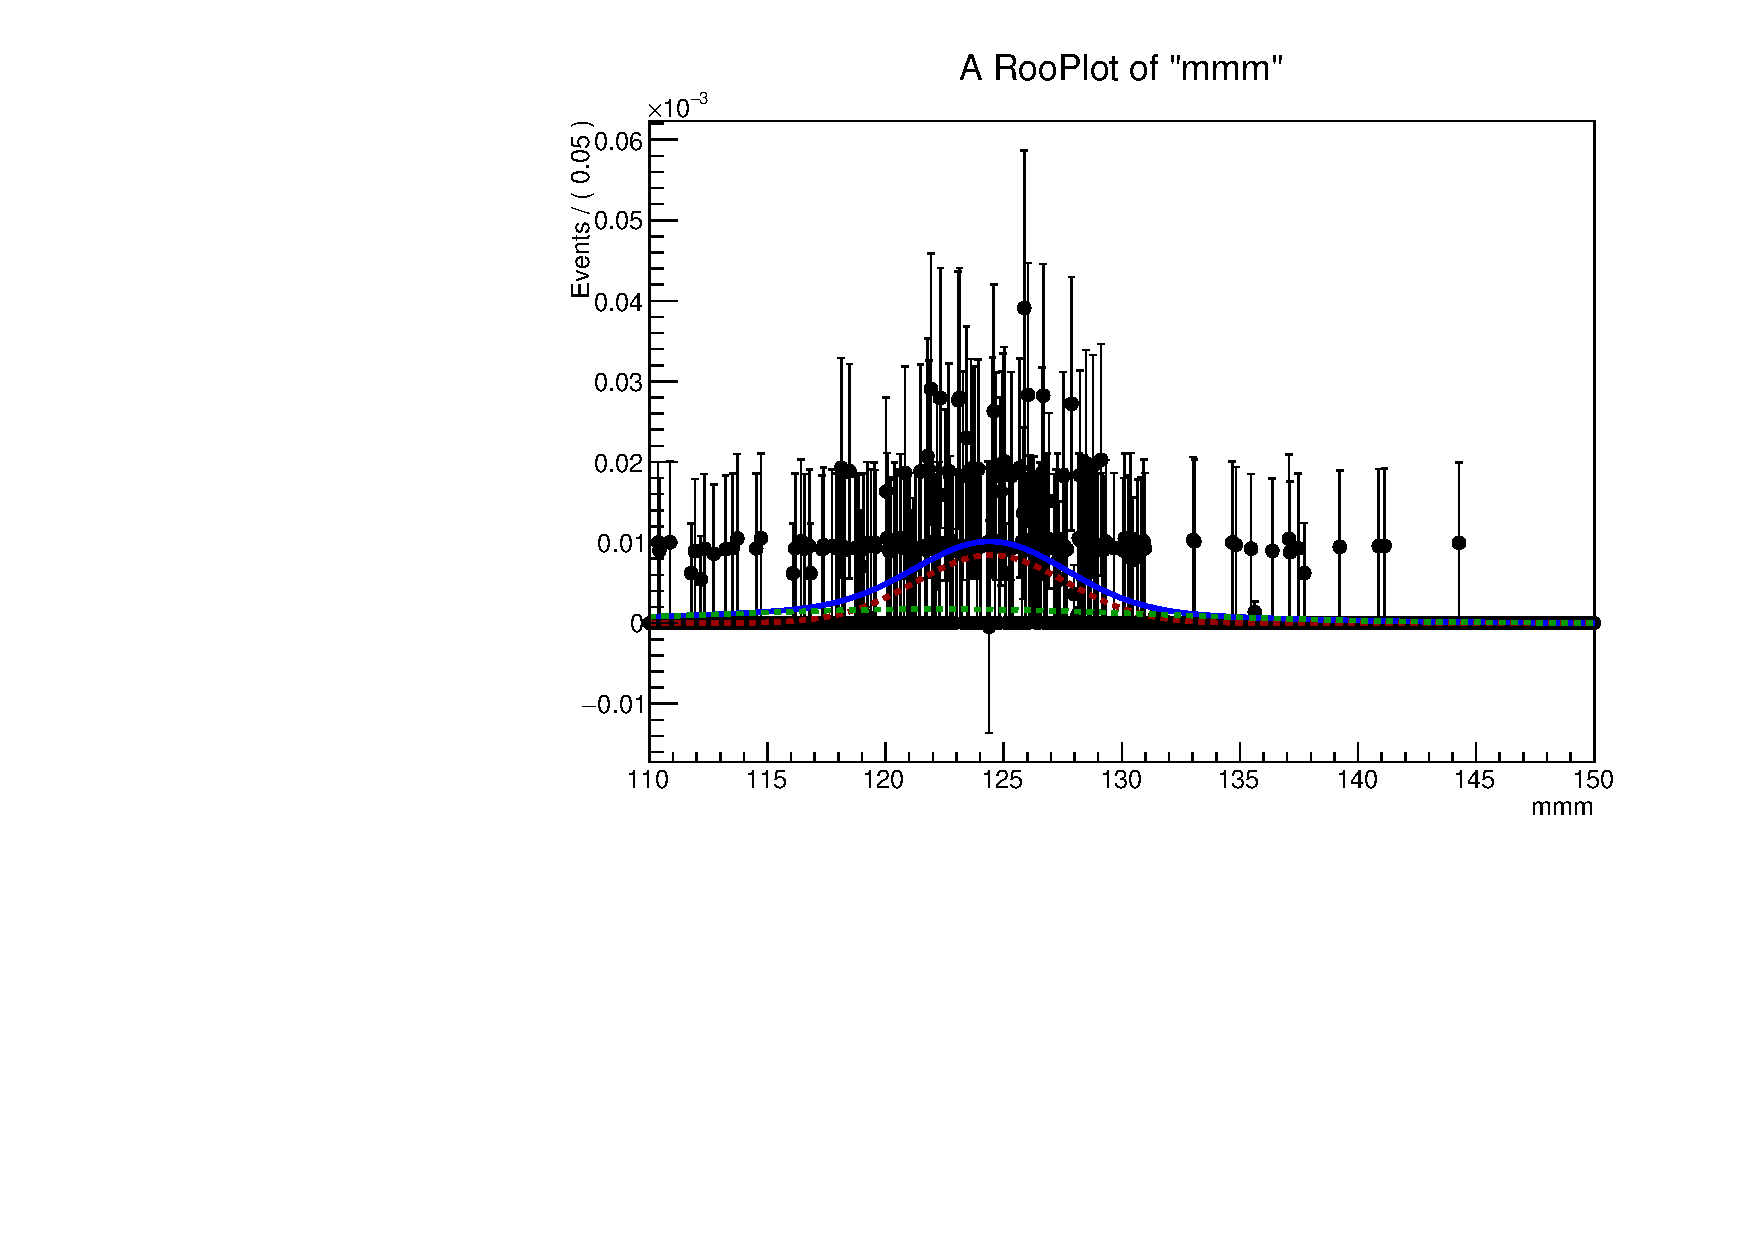
\includegraphics[width=.47\textwidth]{figures/signal_model/AppendixBdt/ttH/125/fit_mh_125_ttH_cat3.pdf}
}
 \\
\hline
\parbox{0.47\textwidth}{
\centering
{\bfseries fit-mh-125-ttH-cat4.pdf}
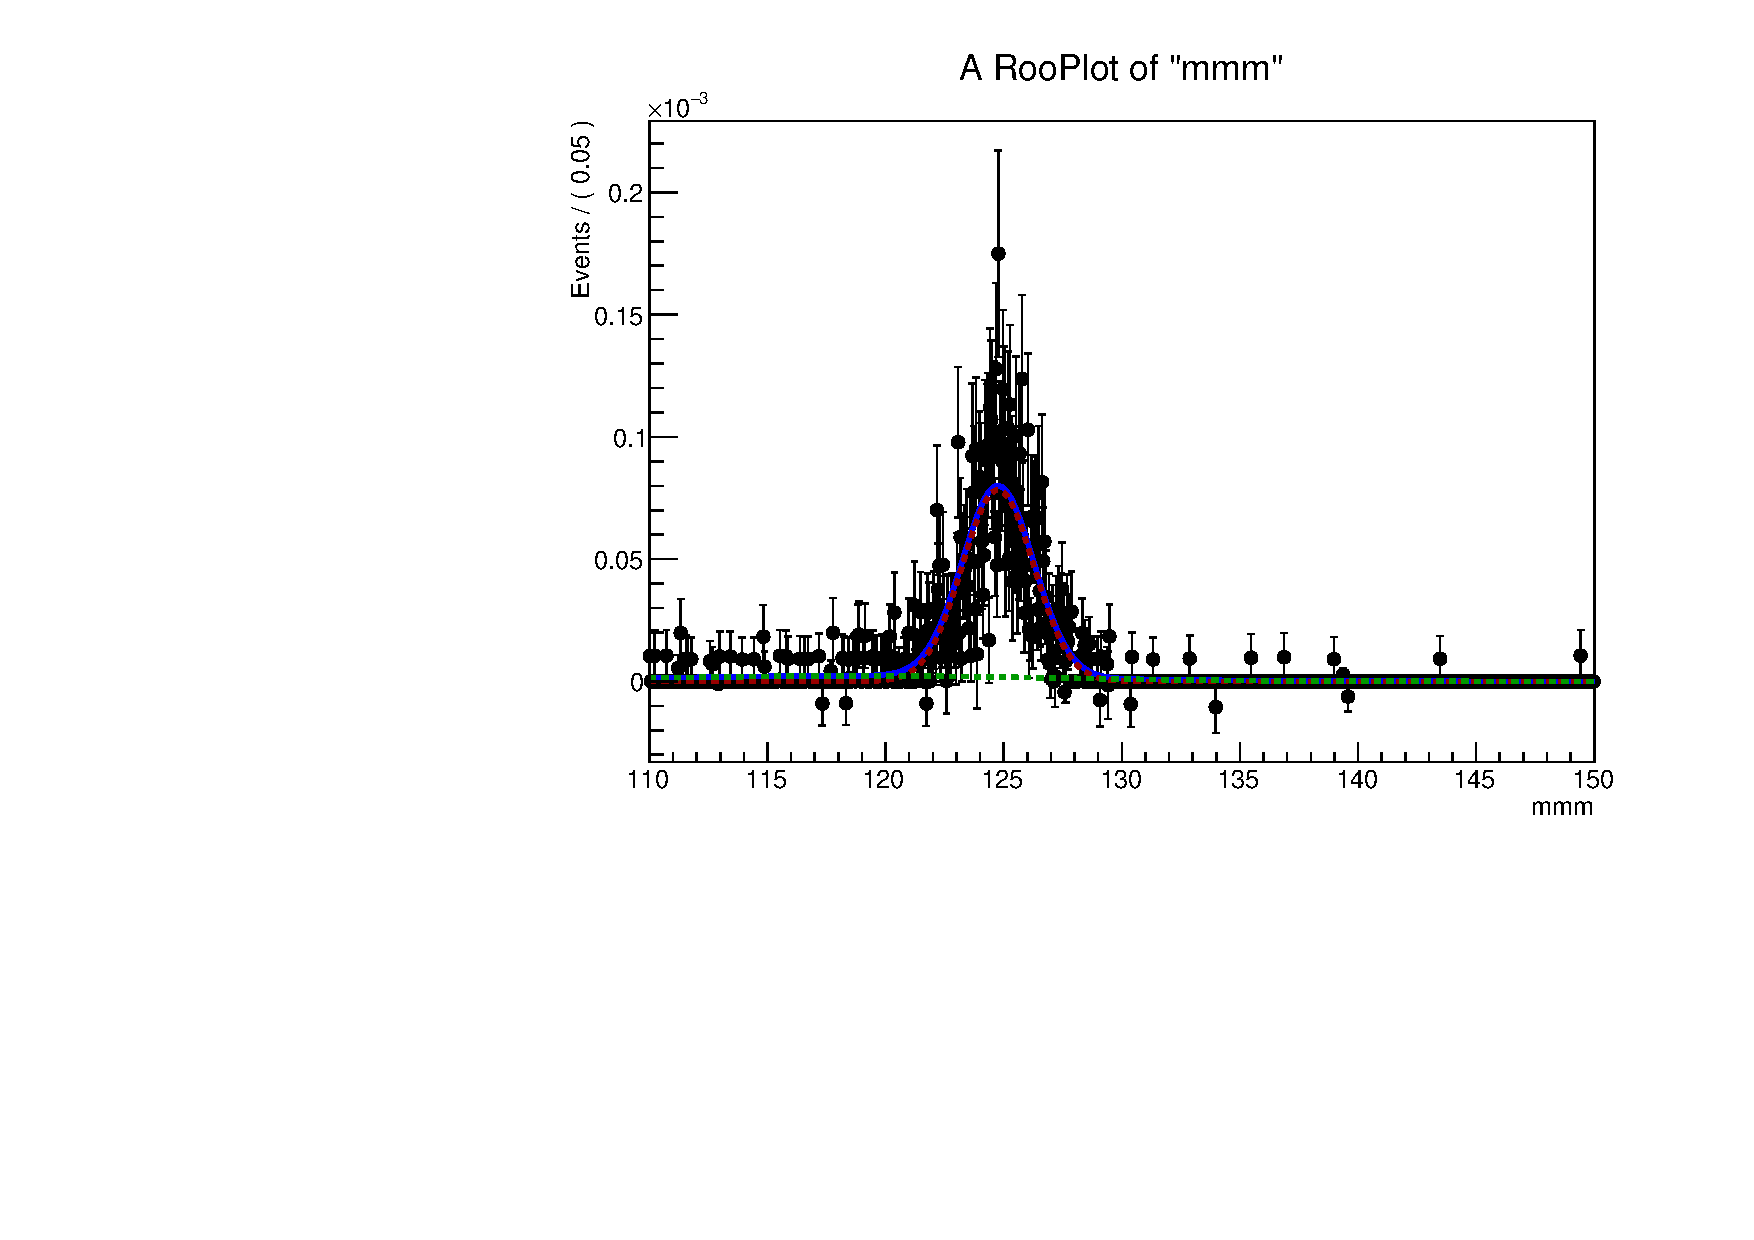
\includegraphics[width=.47\textwidth]{figures/signal_model/AppendixBdt/ttH/125/fit_mh_125_ttH_cat4.pdf}
}
 & \parbox{0.47\textwidth}{
\centering
{\bfseries fit-mh-125-ttH-cat5.pdf}
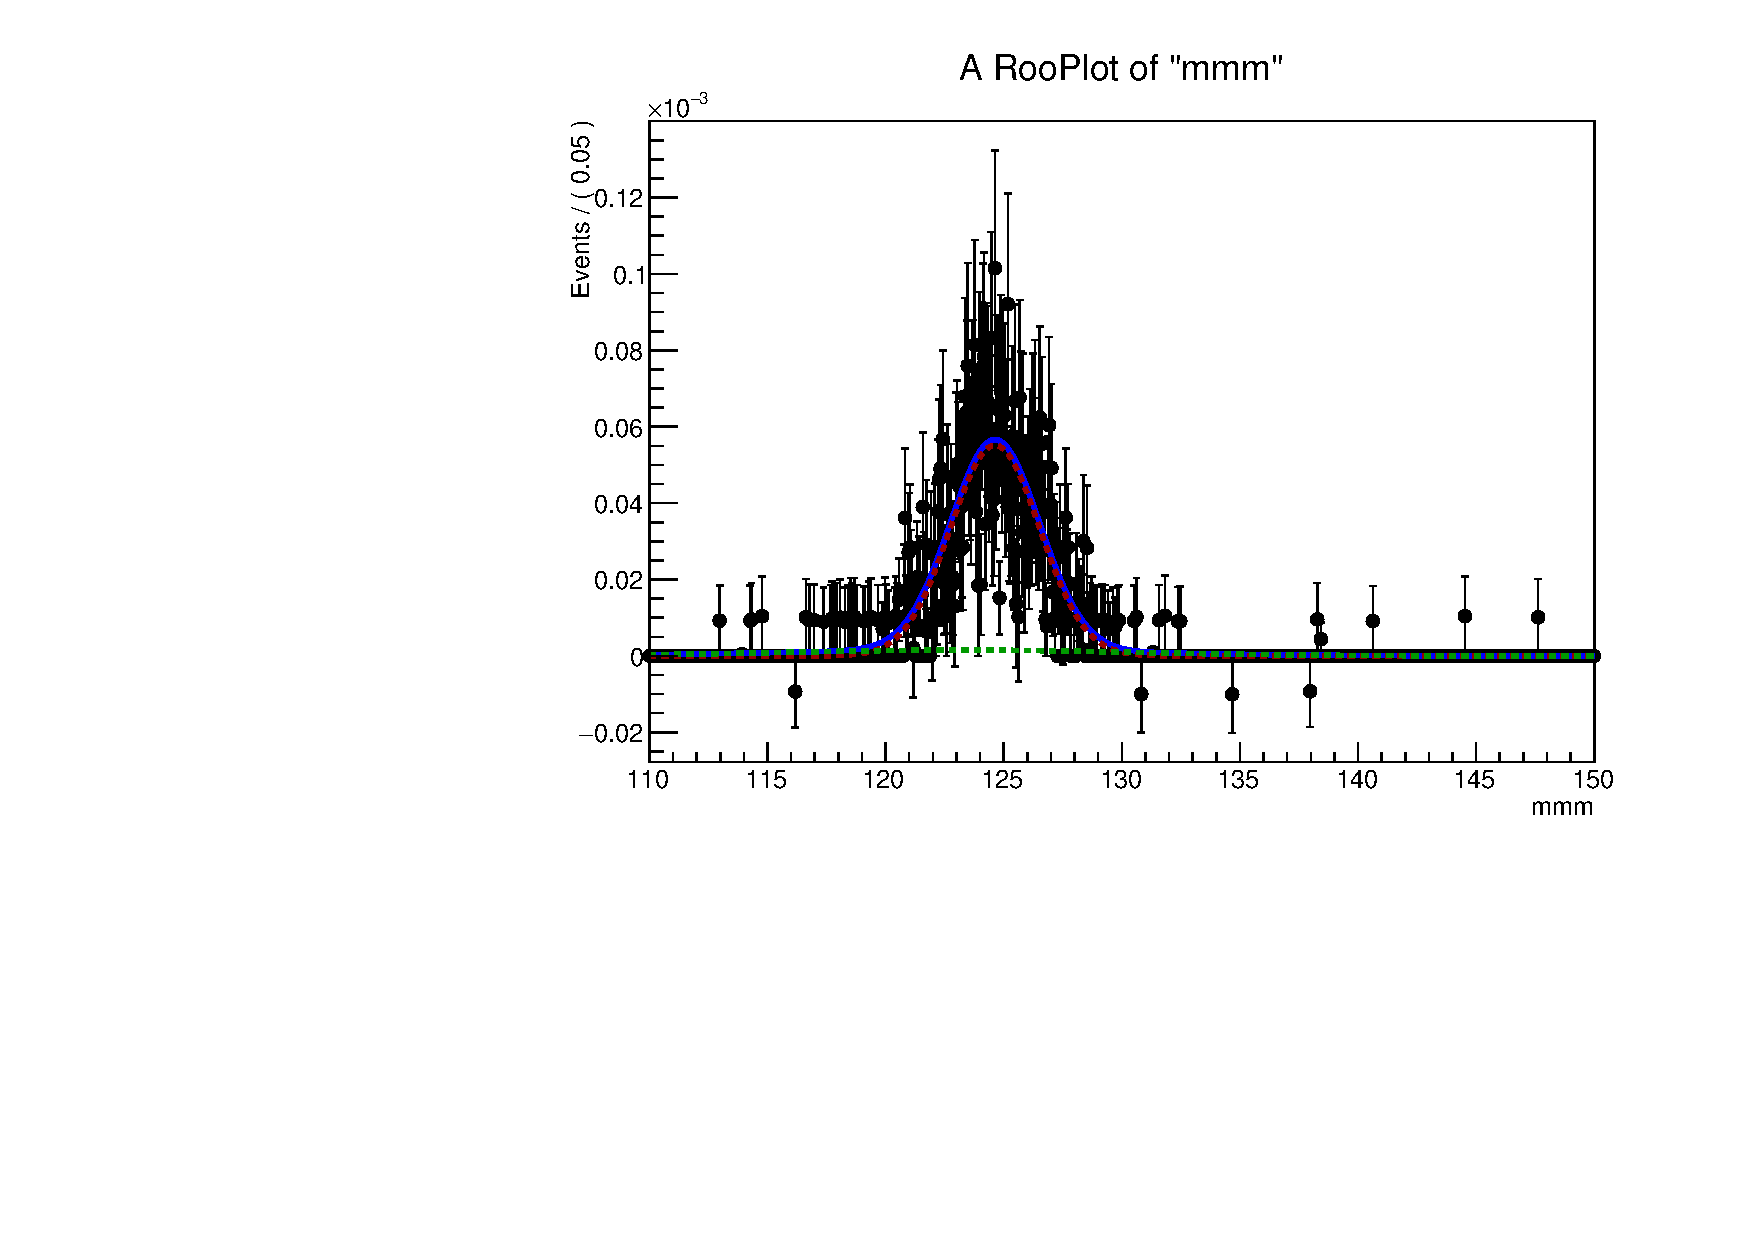
\includegraphics[width=.47\textwidth]{figures/signal_model/AppendixBdt/ttH/125/fit_mh_125_ttH_cat5.pdf}
}
 \\
\hline
\parbox{0.47\textwidth}{
\centering
{\bfseries fit-mh-125-ttH-cat6.pdf}
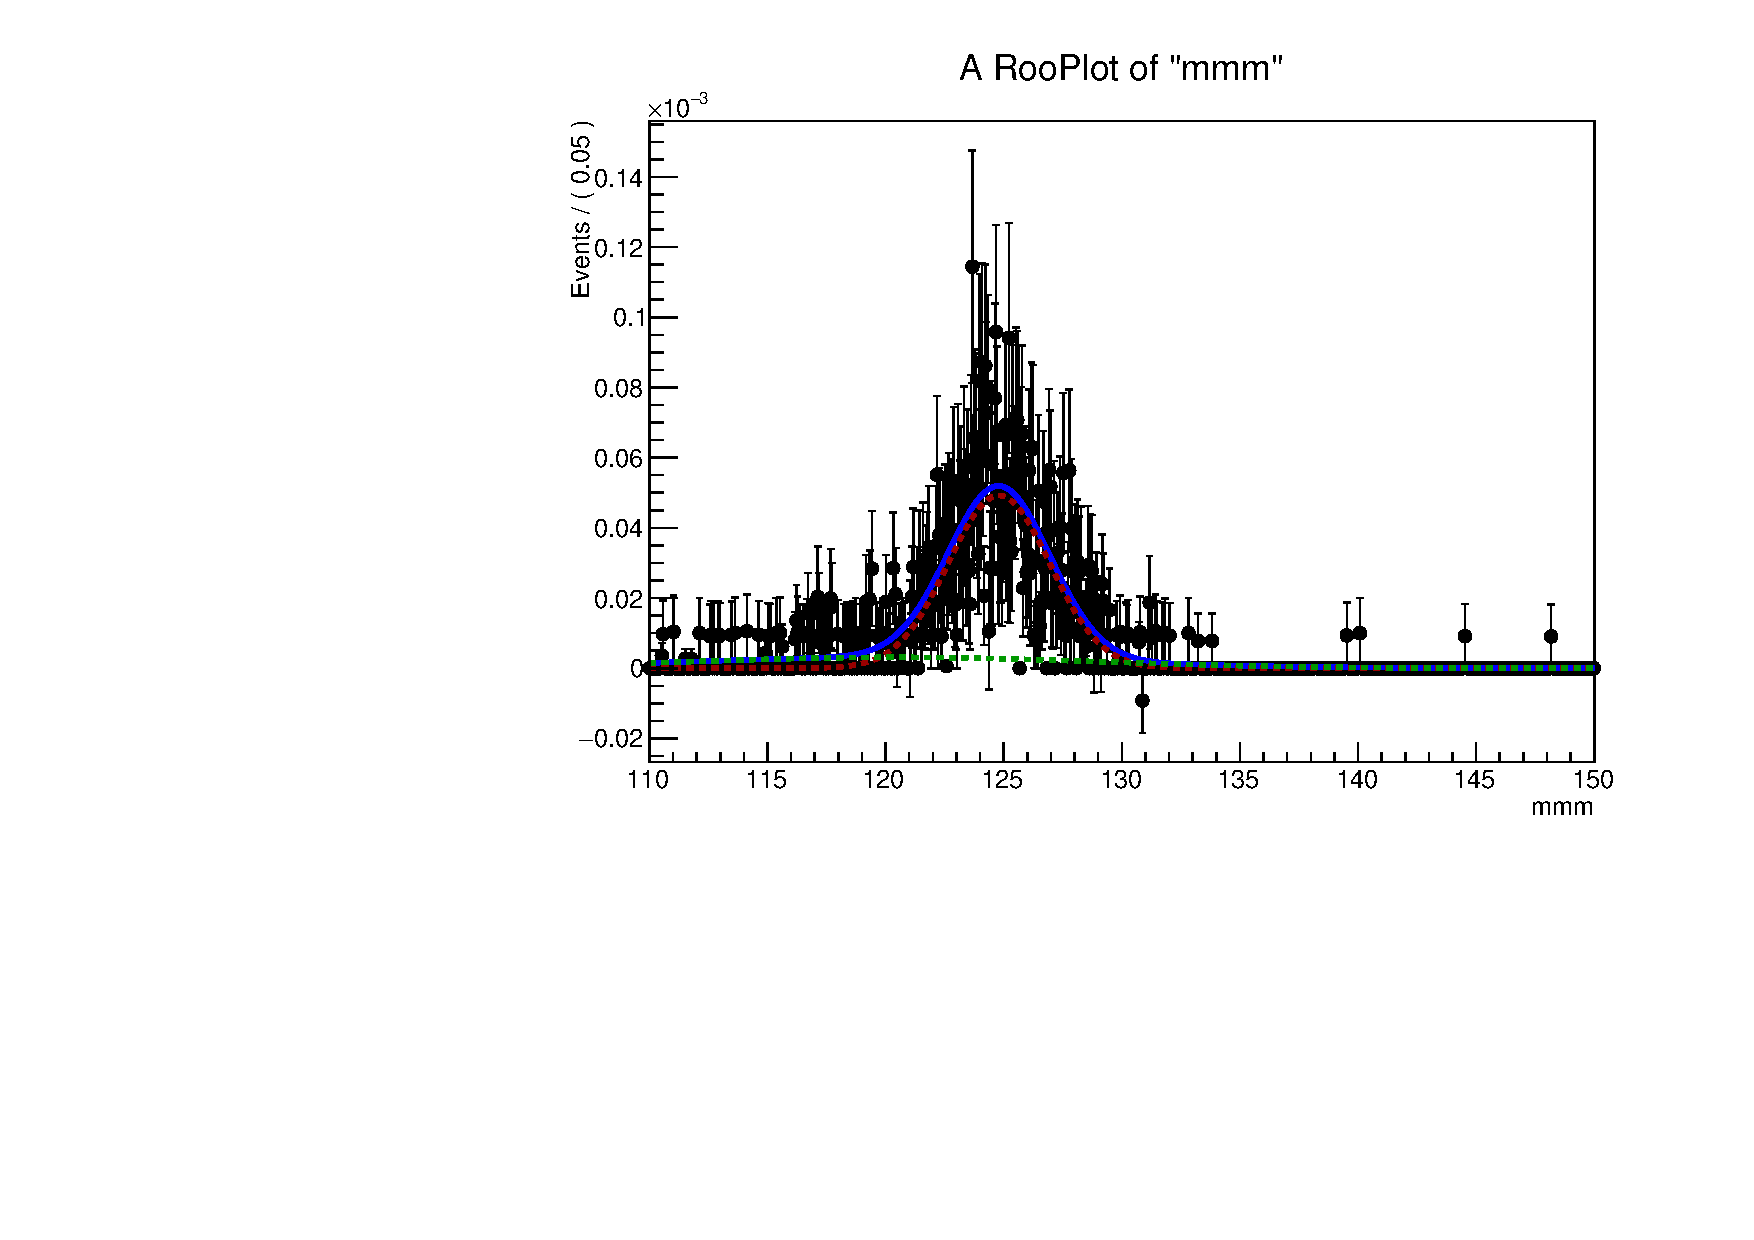
\includegraphics[width=.47\textwidth]{figures/signal_model/AppendixBdt/ttH/125/fit_mh_125_ttH_cat6.pdf}
}
 & \parbox{0.47\textwidth}{
\centering
{\bfseries fit-mh-125-ttH-cat7.pdf}
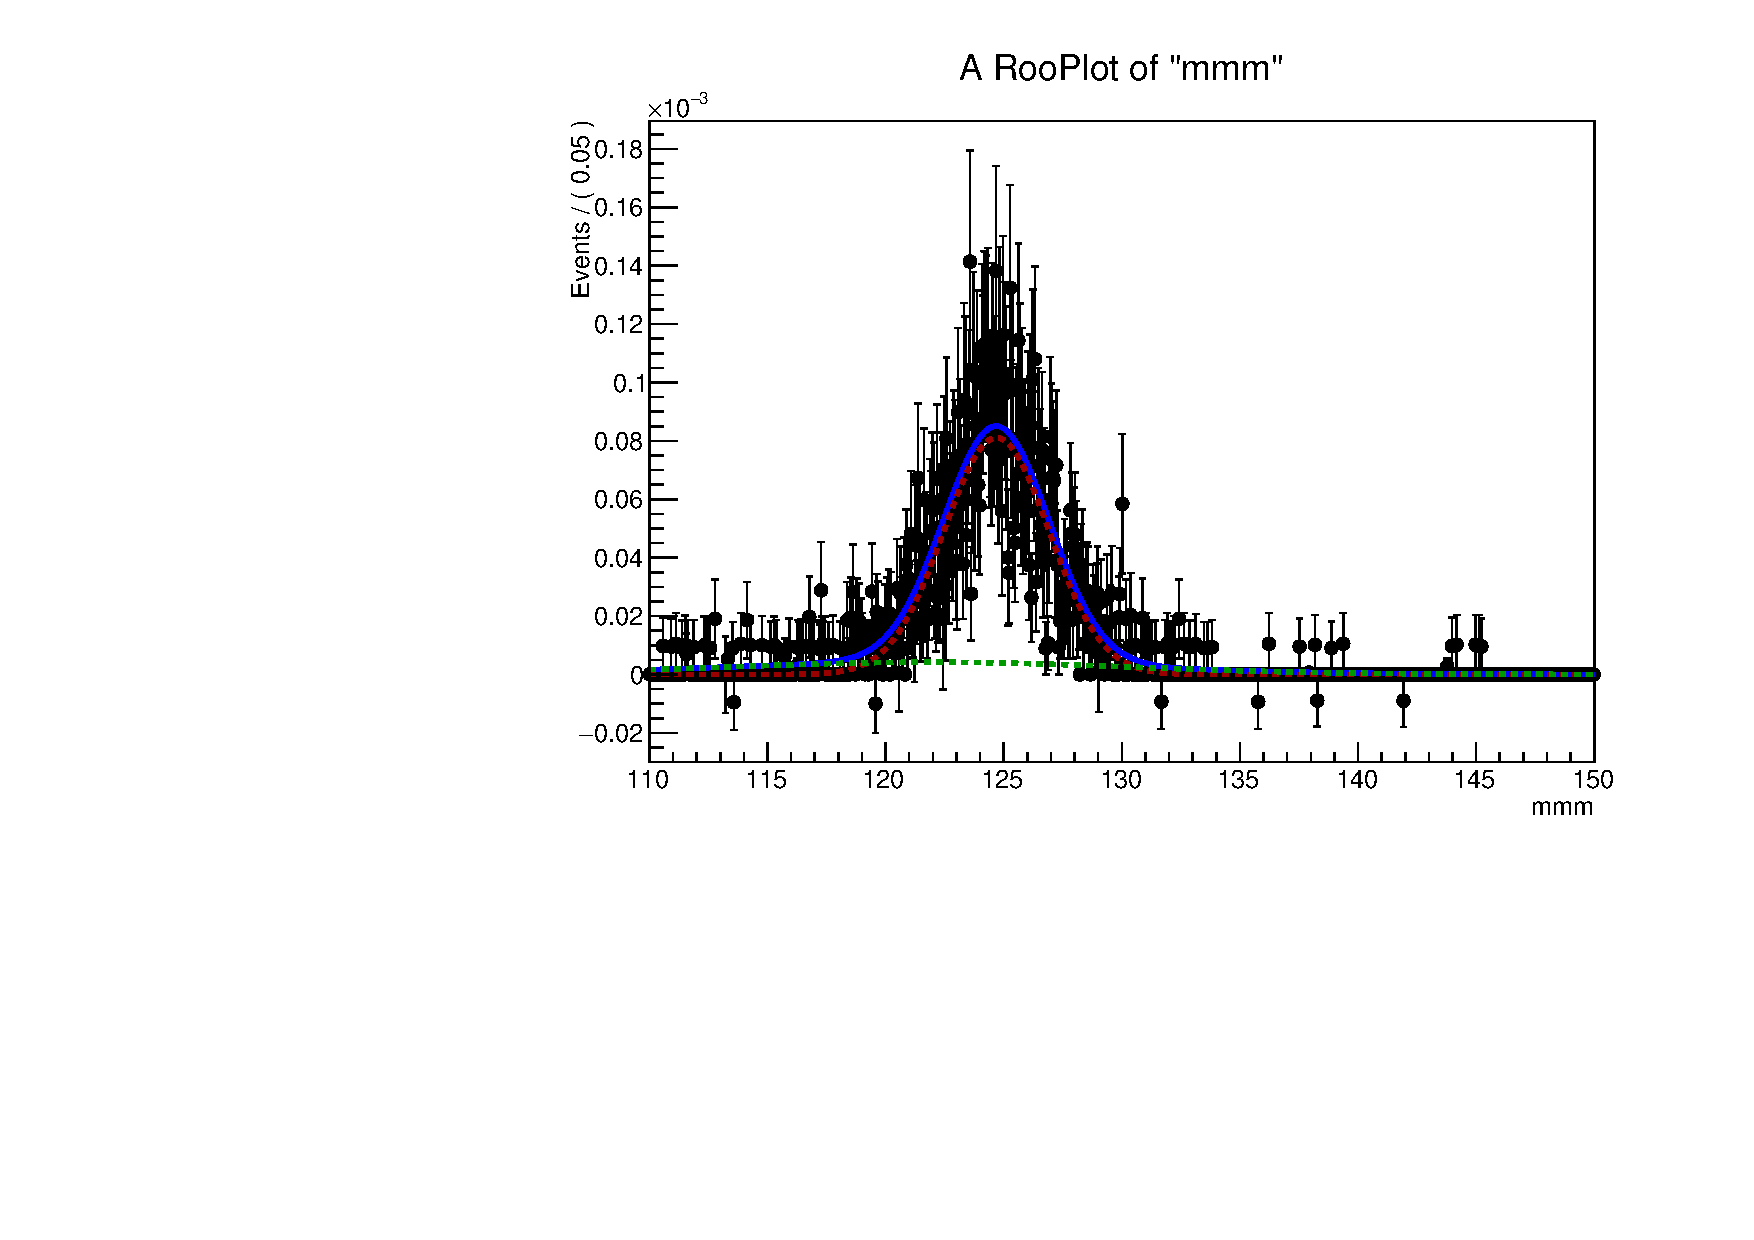
\includegraphics[width=.47\textwidth]{figures/signal_model/AppendixBdt/ttH/125/fit_mh_125_ttH_cat7.pdf}
}
 \\
\hline
\parbox{0.47\textwidth}{
\centering
{\bfseries fit-mh-125-ttH-cat8.pdf}
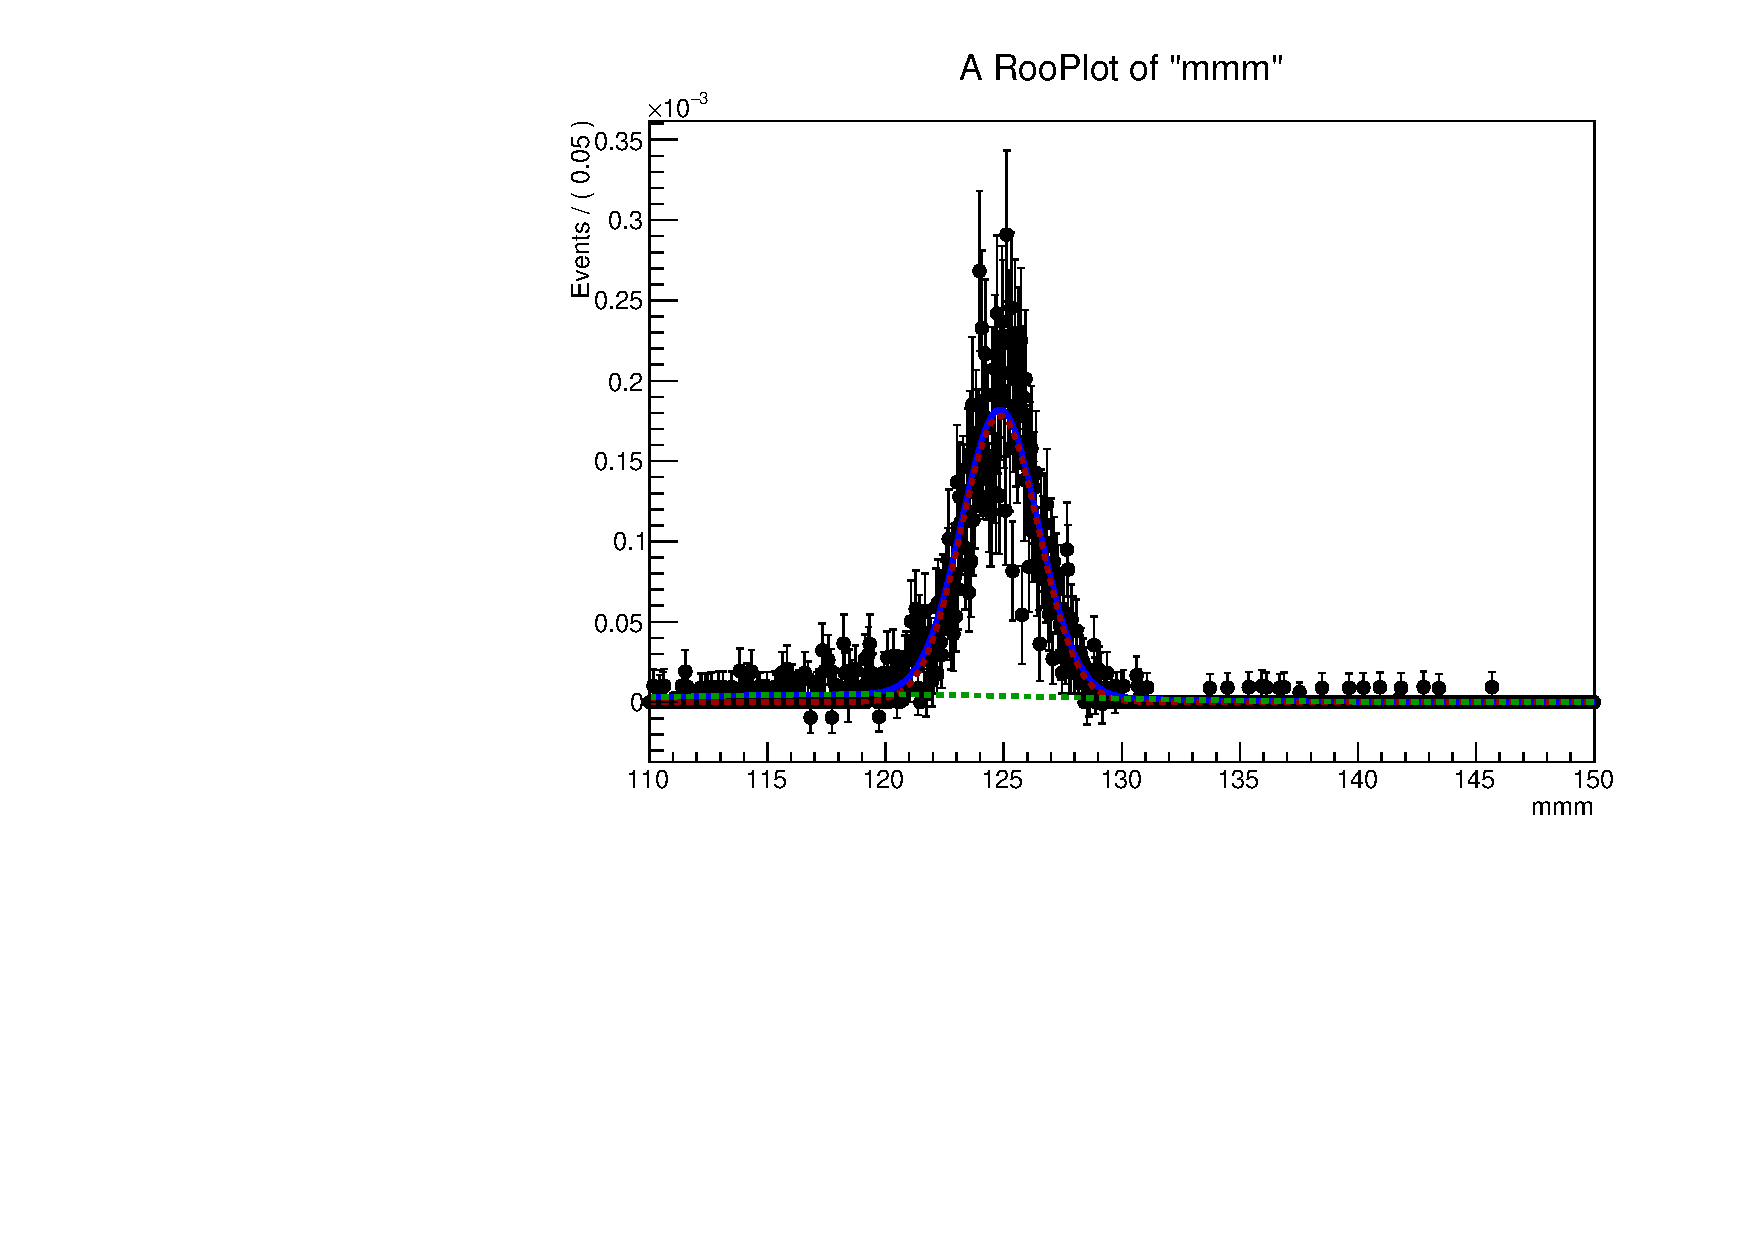
\includegraphics[width=.47\textwidth]{figures/signal_model/AppendixBdt/ttH/125/fit_mh_125_ttH_cat8.pdf}
}
 & \parbox{0.47\textwidth}{
\centering
{\bfseries fit-mh-125-ttH-cat9.pdf}
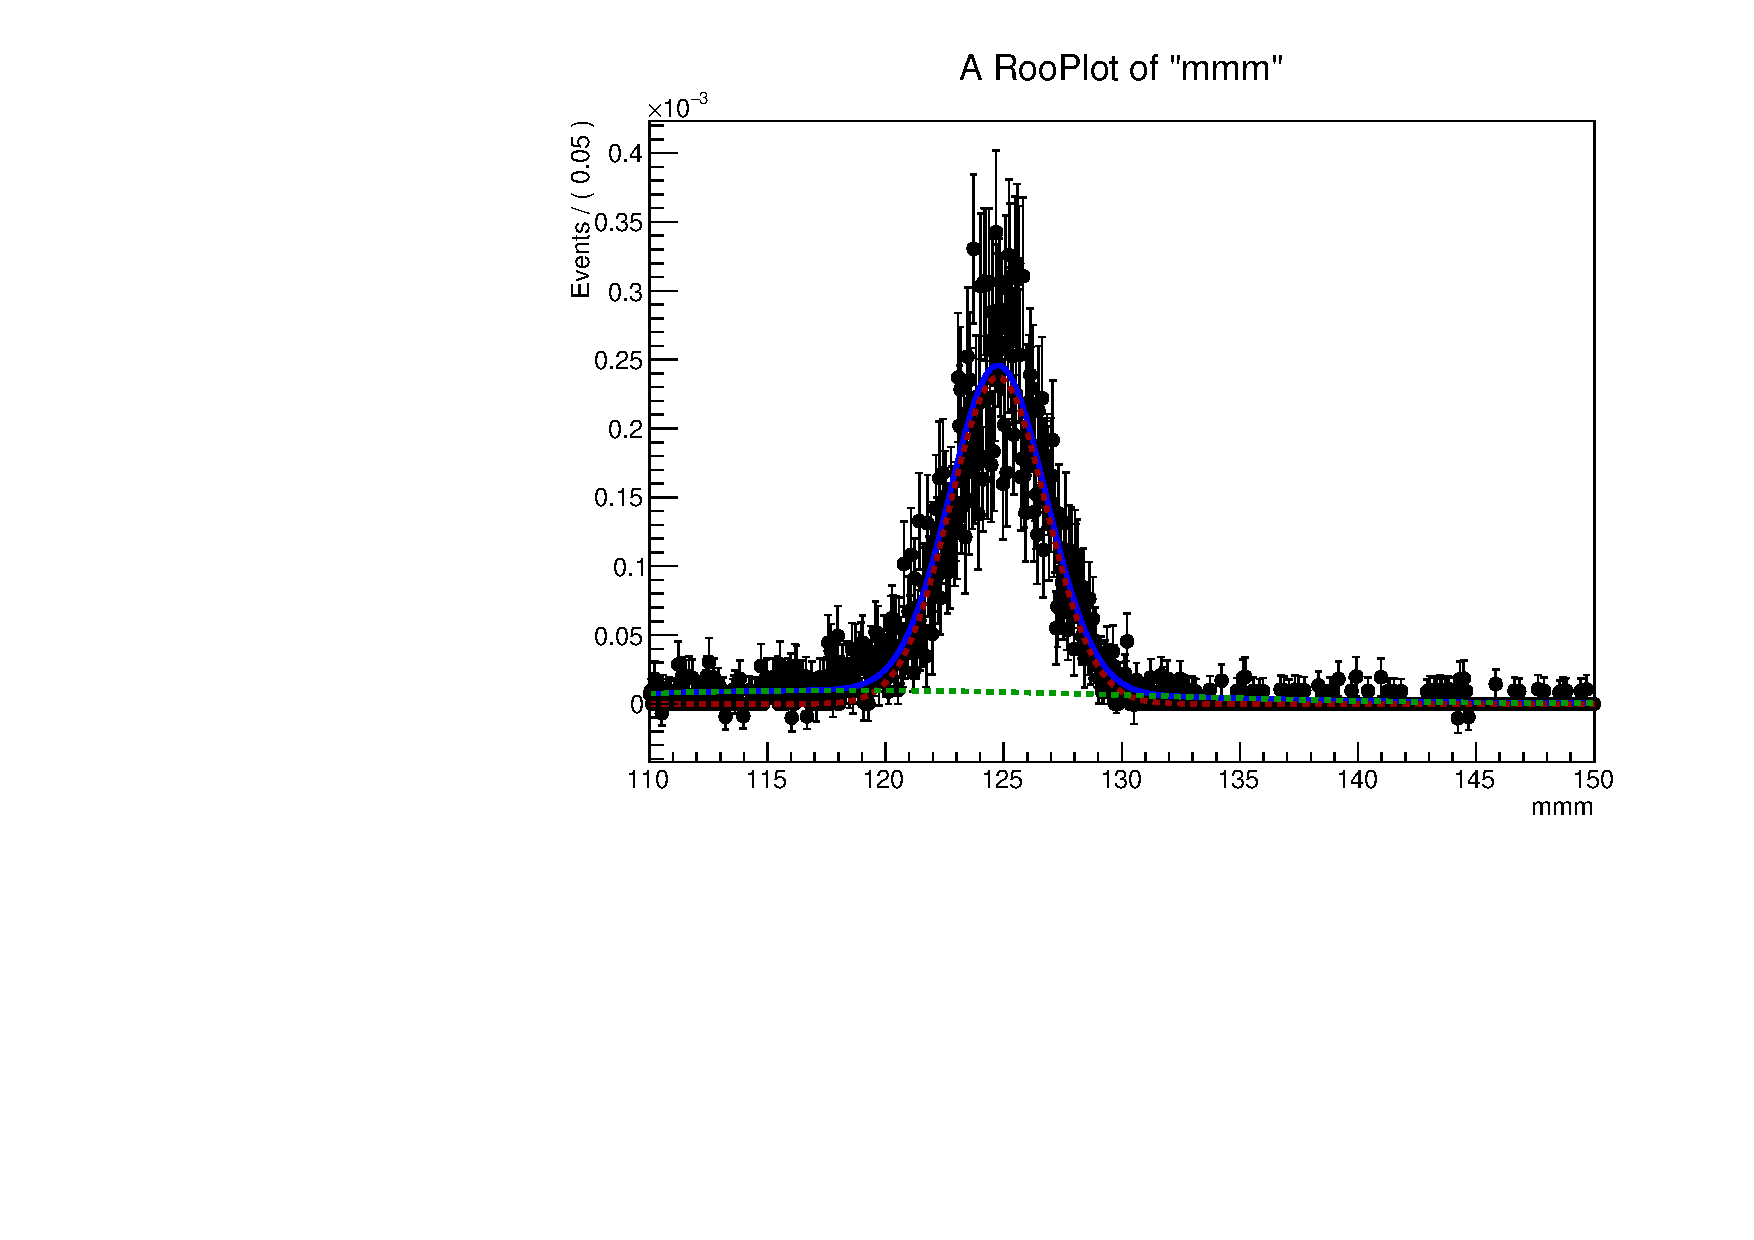
\includegraphics[width=.47\textwidth]{figures/signal_model/AppendixBdt/ttH/125/fit_mh_125_ttH_cat9.pdf}
}
 \\
\hline
\parbox{0.47\textwidth}{
\centering
{\bfseries fit-mh-125-ttH-cat10.pdf}
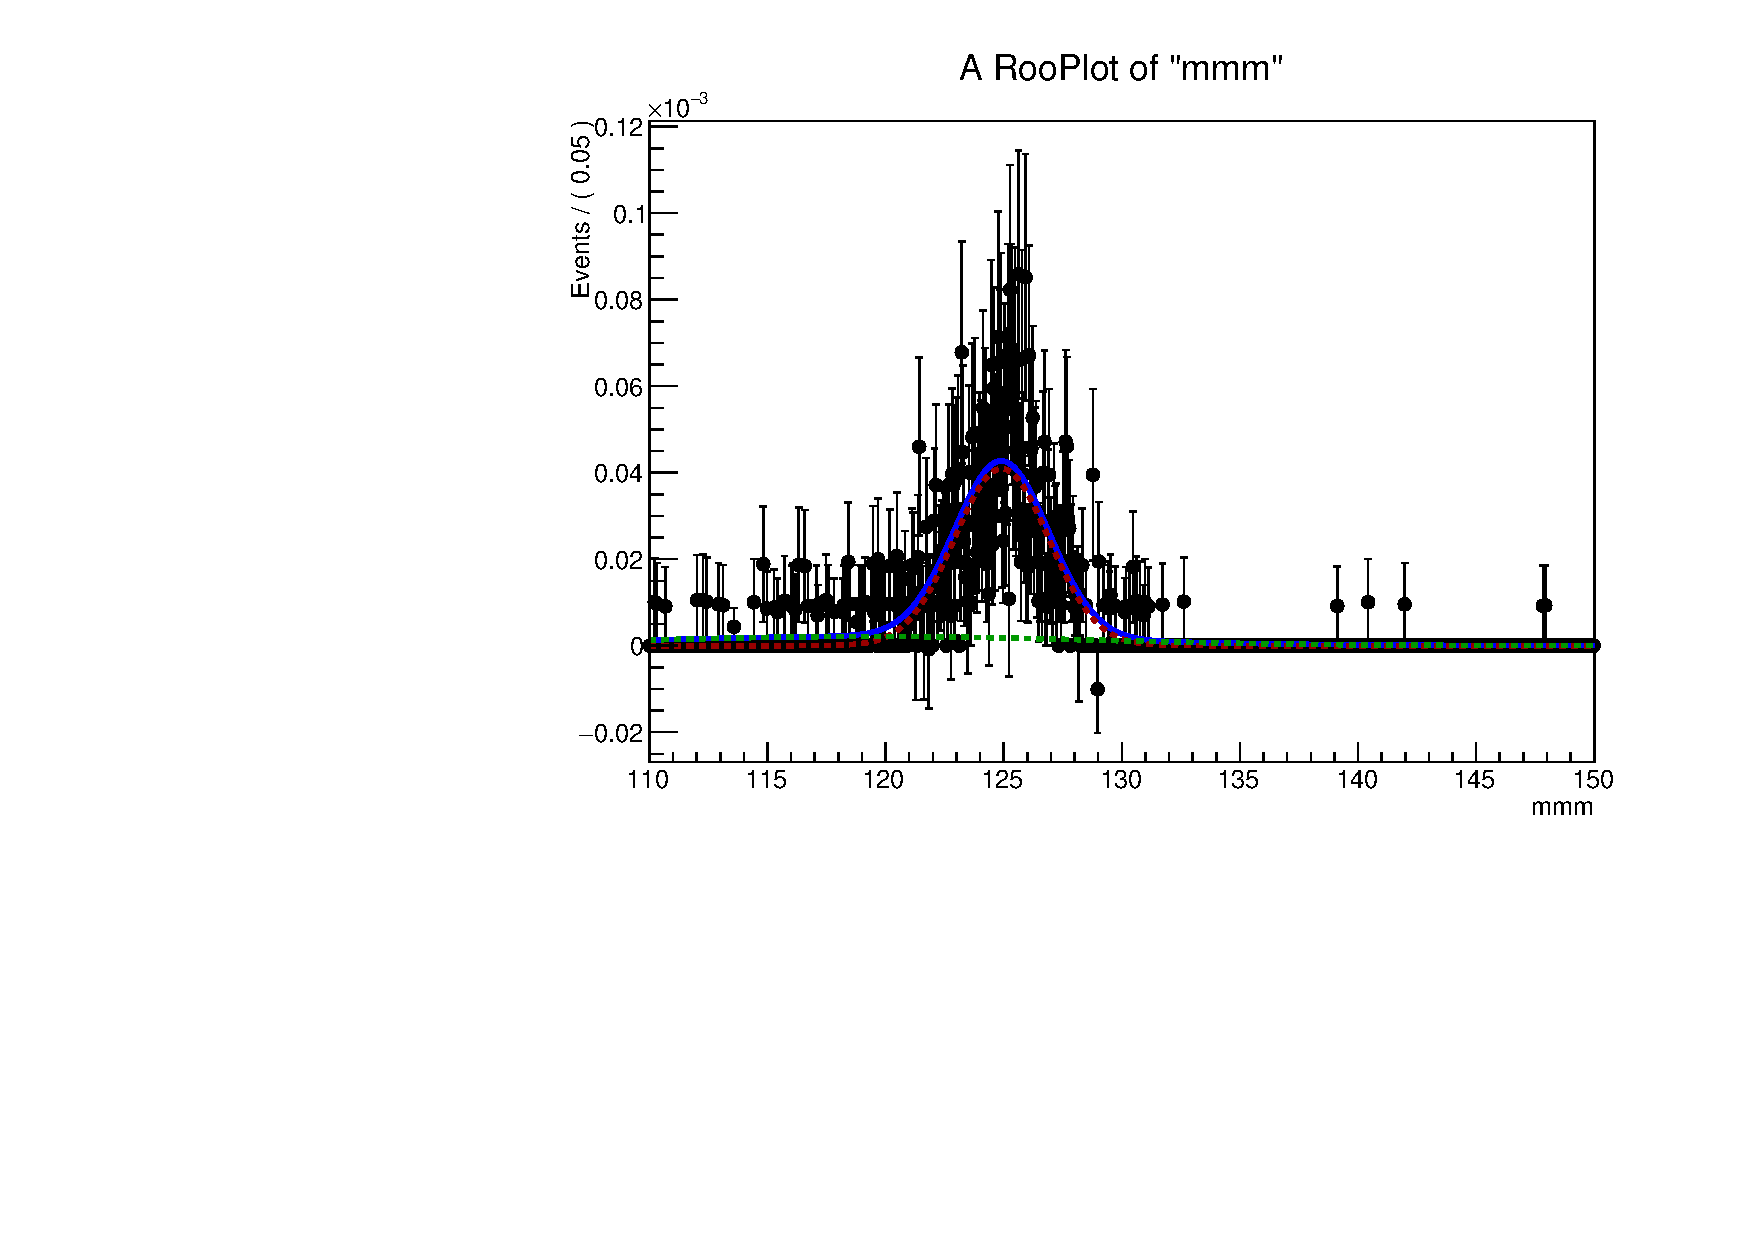
\includegraphics[width=.47\textwidth]{figures/signal_model/AppendixBdt/ttH/125/fit_mh_125_ttH_cat10.pdf}
}
 & \parbox{0.47\textwidth}{
\centering
{\bfseries fit-mh-125-ttH-cat11.pdf}
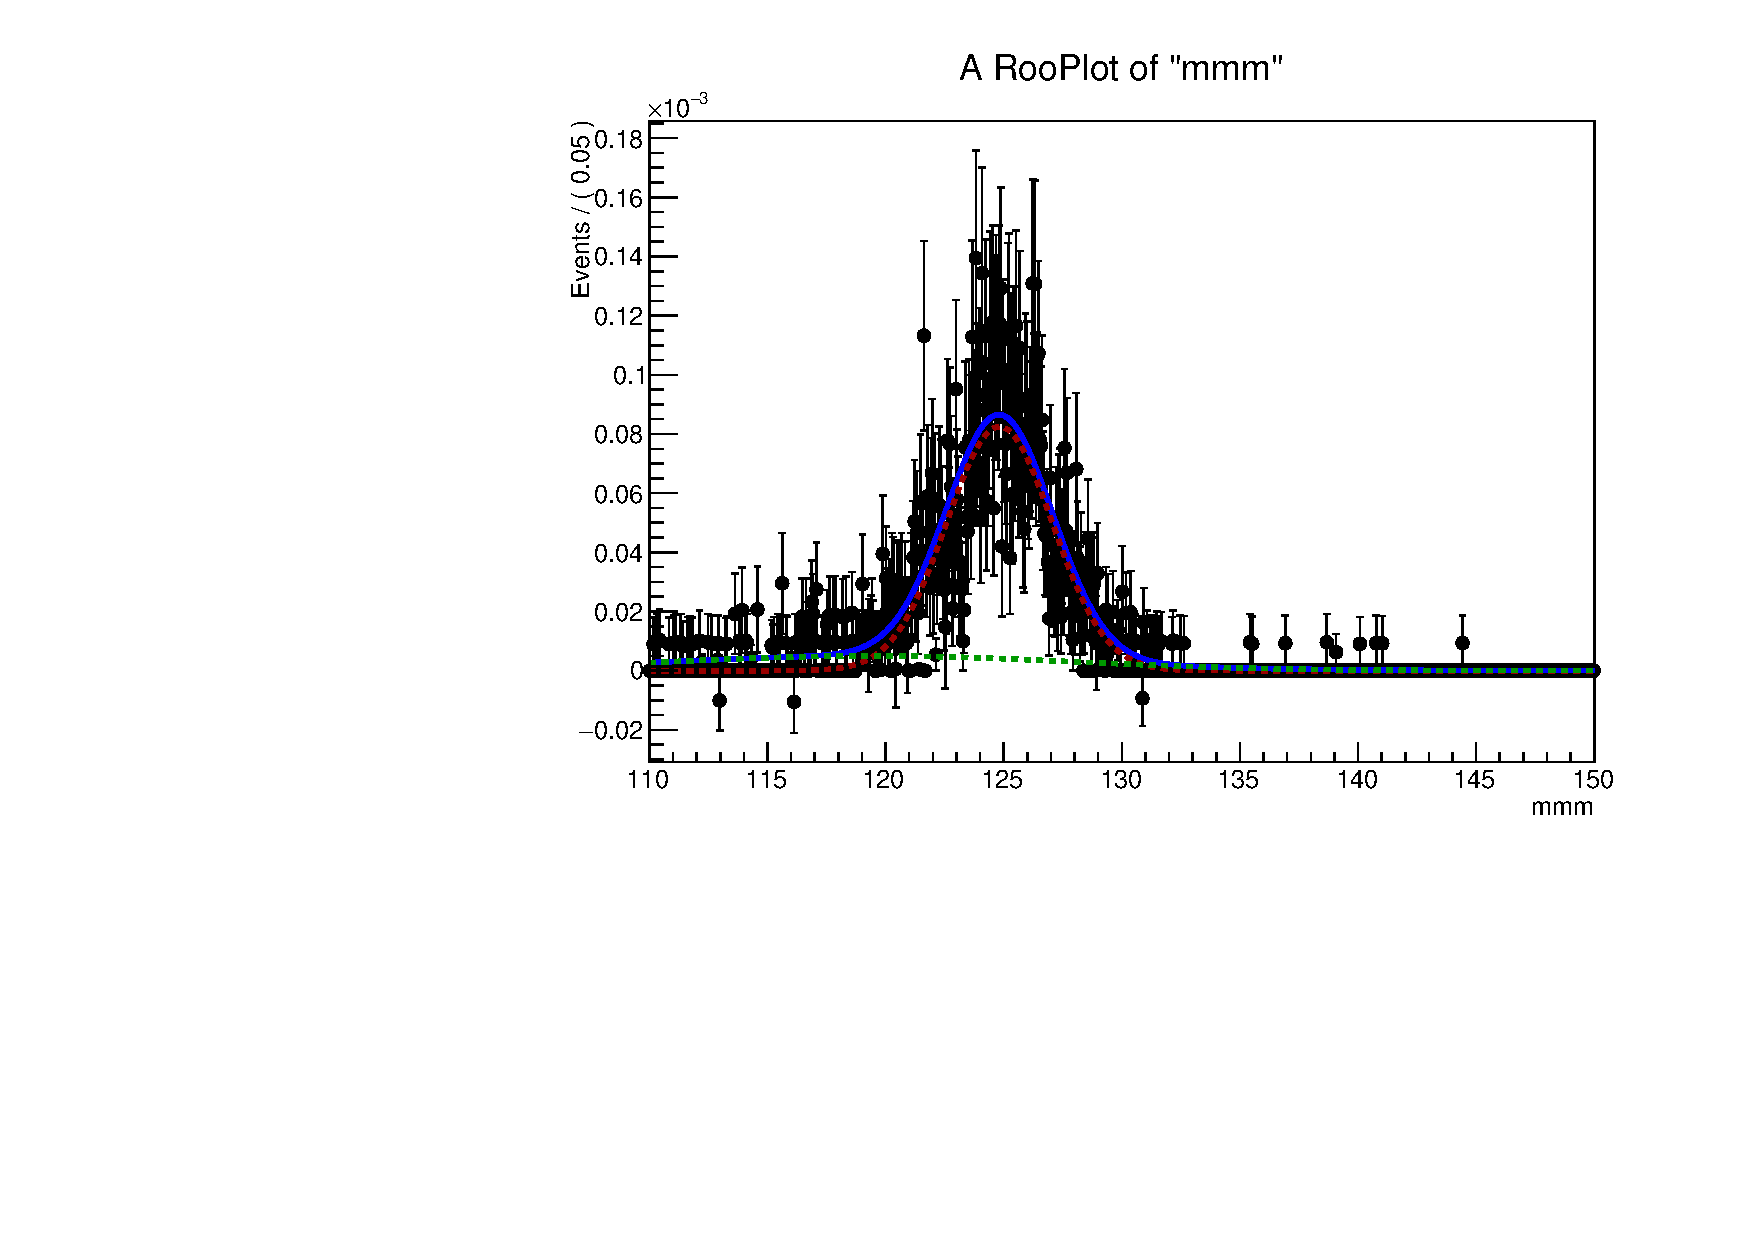
\includegraphics[width=.47\textwidth]{figures/signal_model/AppendixBdt/ttH/125/fit_mh_125_ttH_cat11.pdf}
}
 \\
\hline
\parbox{0.47\textwidth}{
\centering
{\bfseries fit-mh-125-ttH-cat12.pdf}
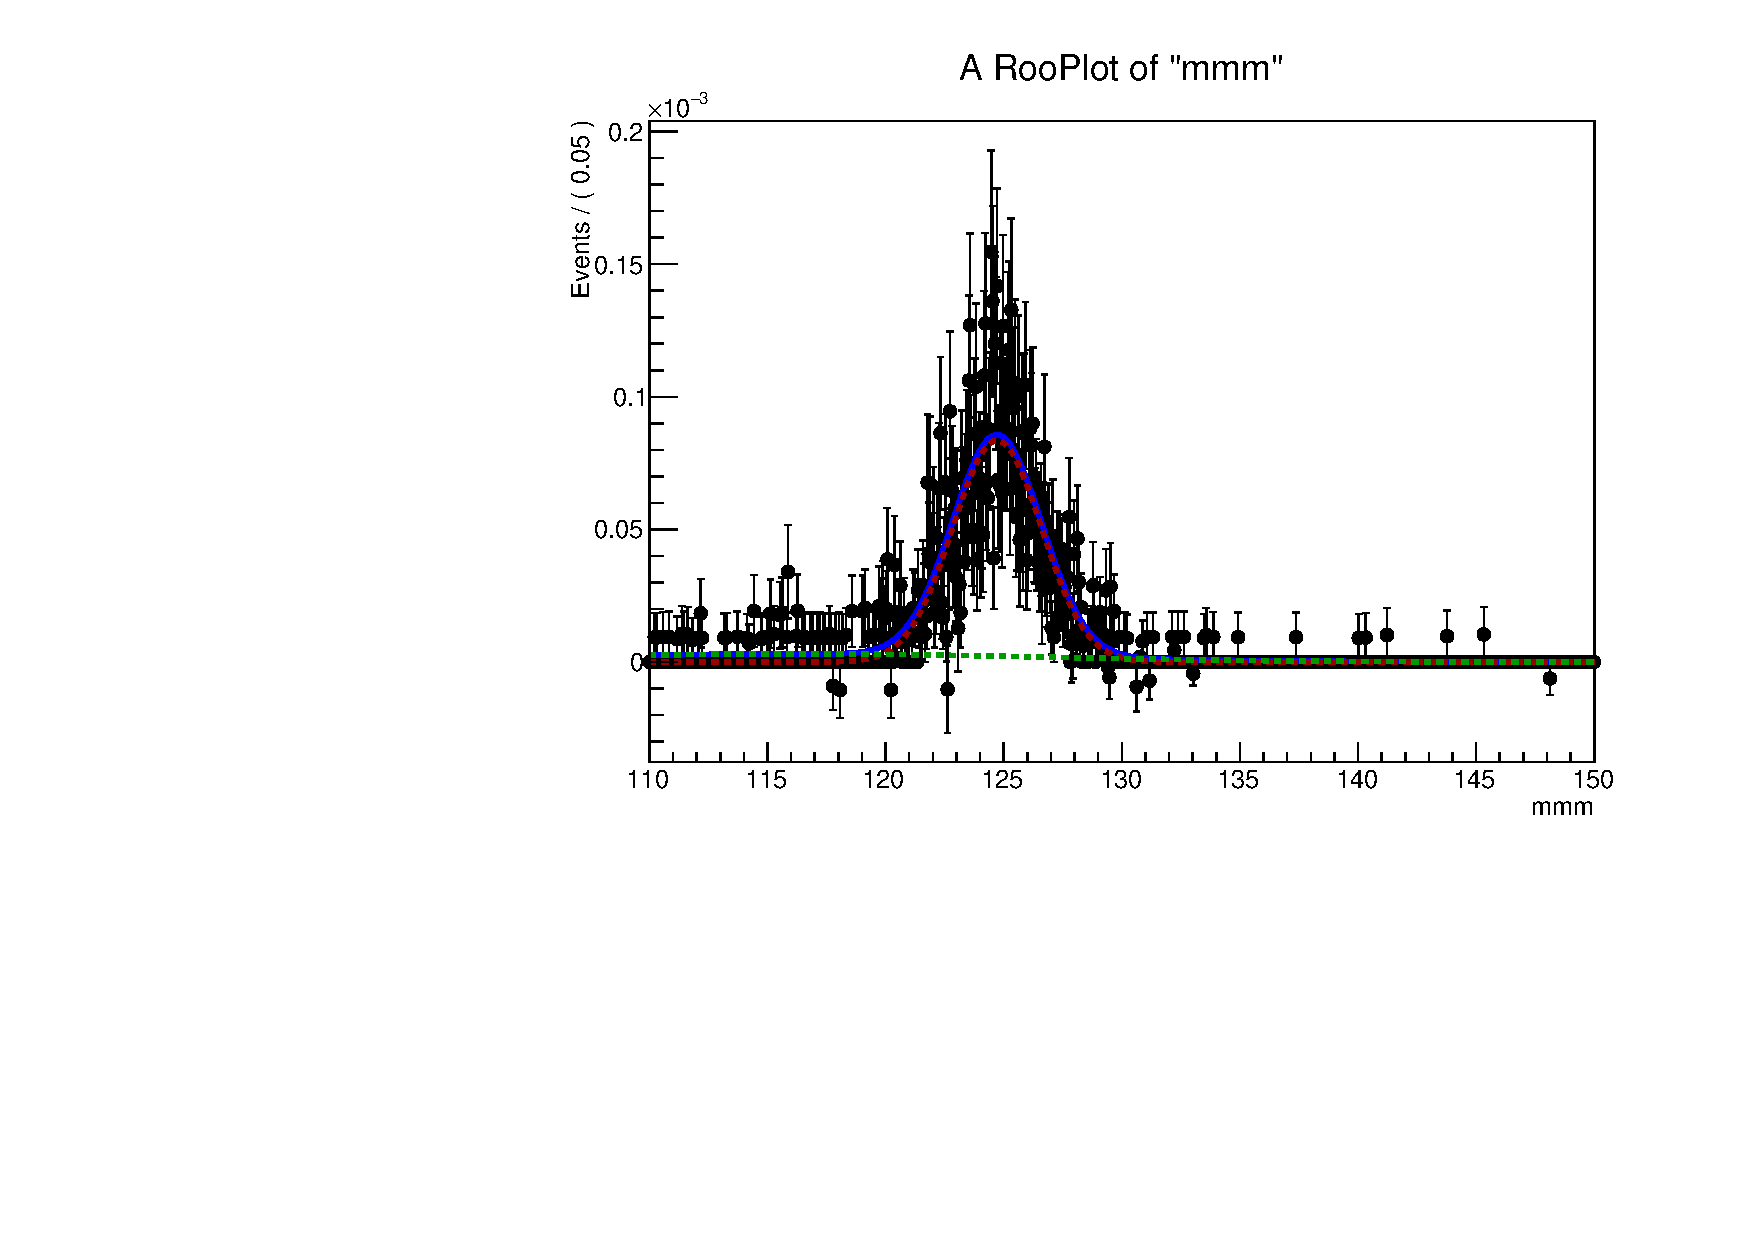
\includegraphics[width=.47\textwidth]{figures/signal_model/AppendixBdt/ttH/125/fit_mh_125_ttH_cat12.pdf}
}
 & \parbox{0.47\textwidth}{
\centering
{\bfseries fit-mh-125-ttH-cat13.pdf}
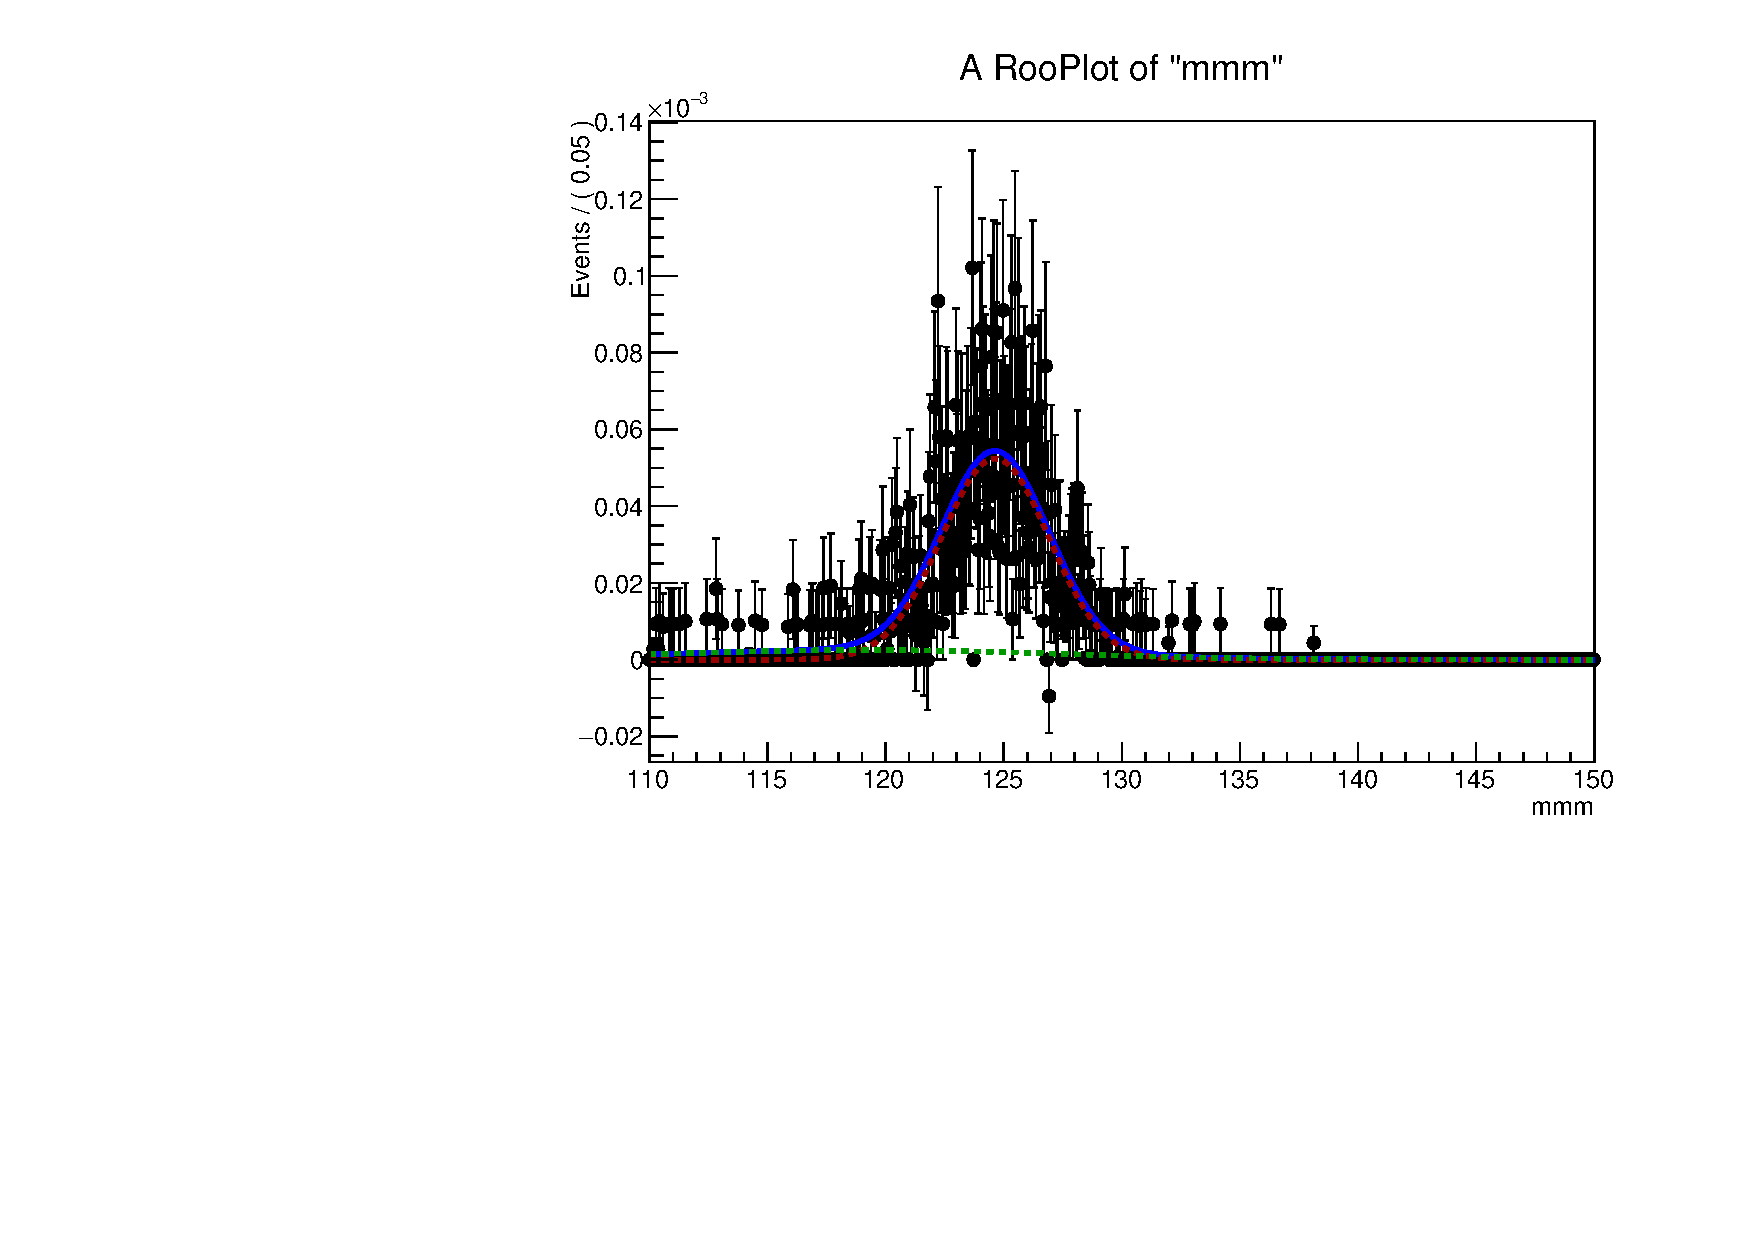
\includegraphics[width=.47\textwidth]{figures/signal_model/AppendixBdt/ttH/125/fit_mh_125_ttH_cat13.pdf}
}
 \\
\hline
\parbox{0.47\textwidth}{
\centering
{\bfseries fit-mh-125-ttH-cat14.pdf}
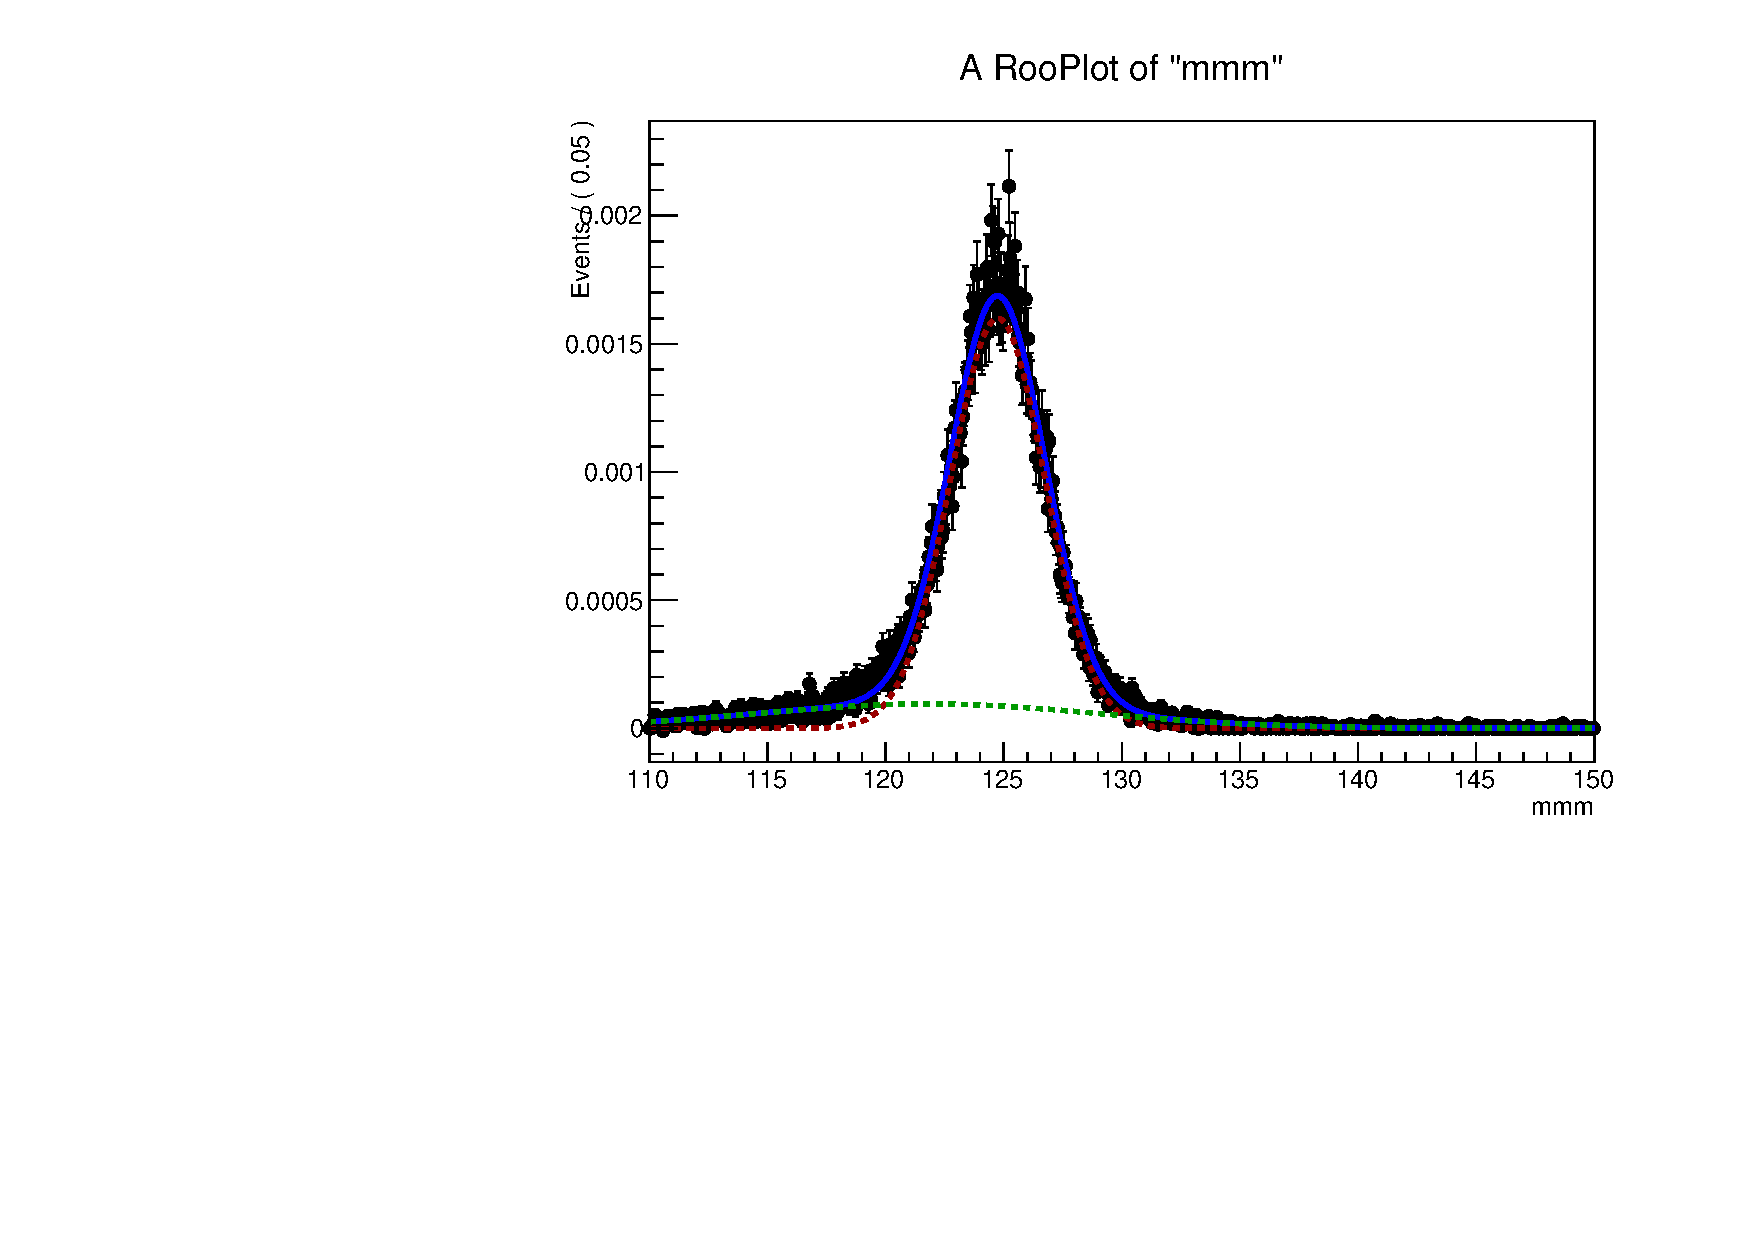
\includegraphics[width=.47\textwidth]{figures/signal_model/AppendixBdt/ttH/125/fit_mh_125_ttH_cat14.pdf}
}
 & \parbox{0.47\textwidth}{
\centering
{\bfseries fit-mh-125-ttH-cat15.pdf}
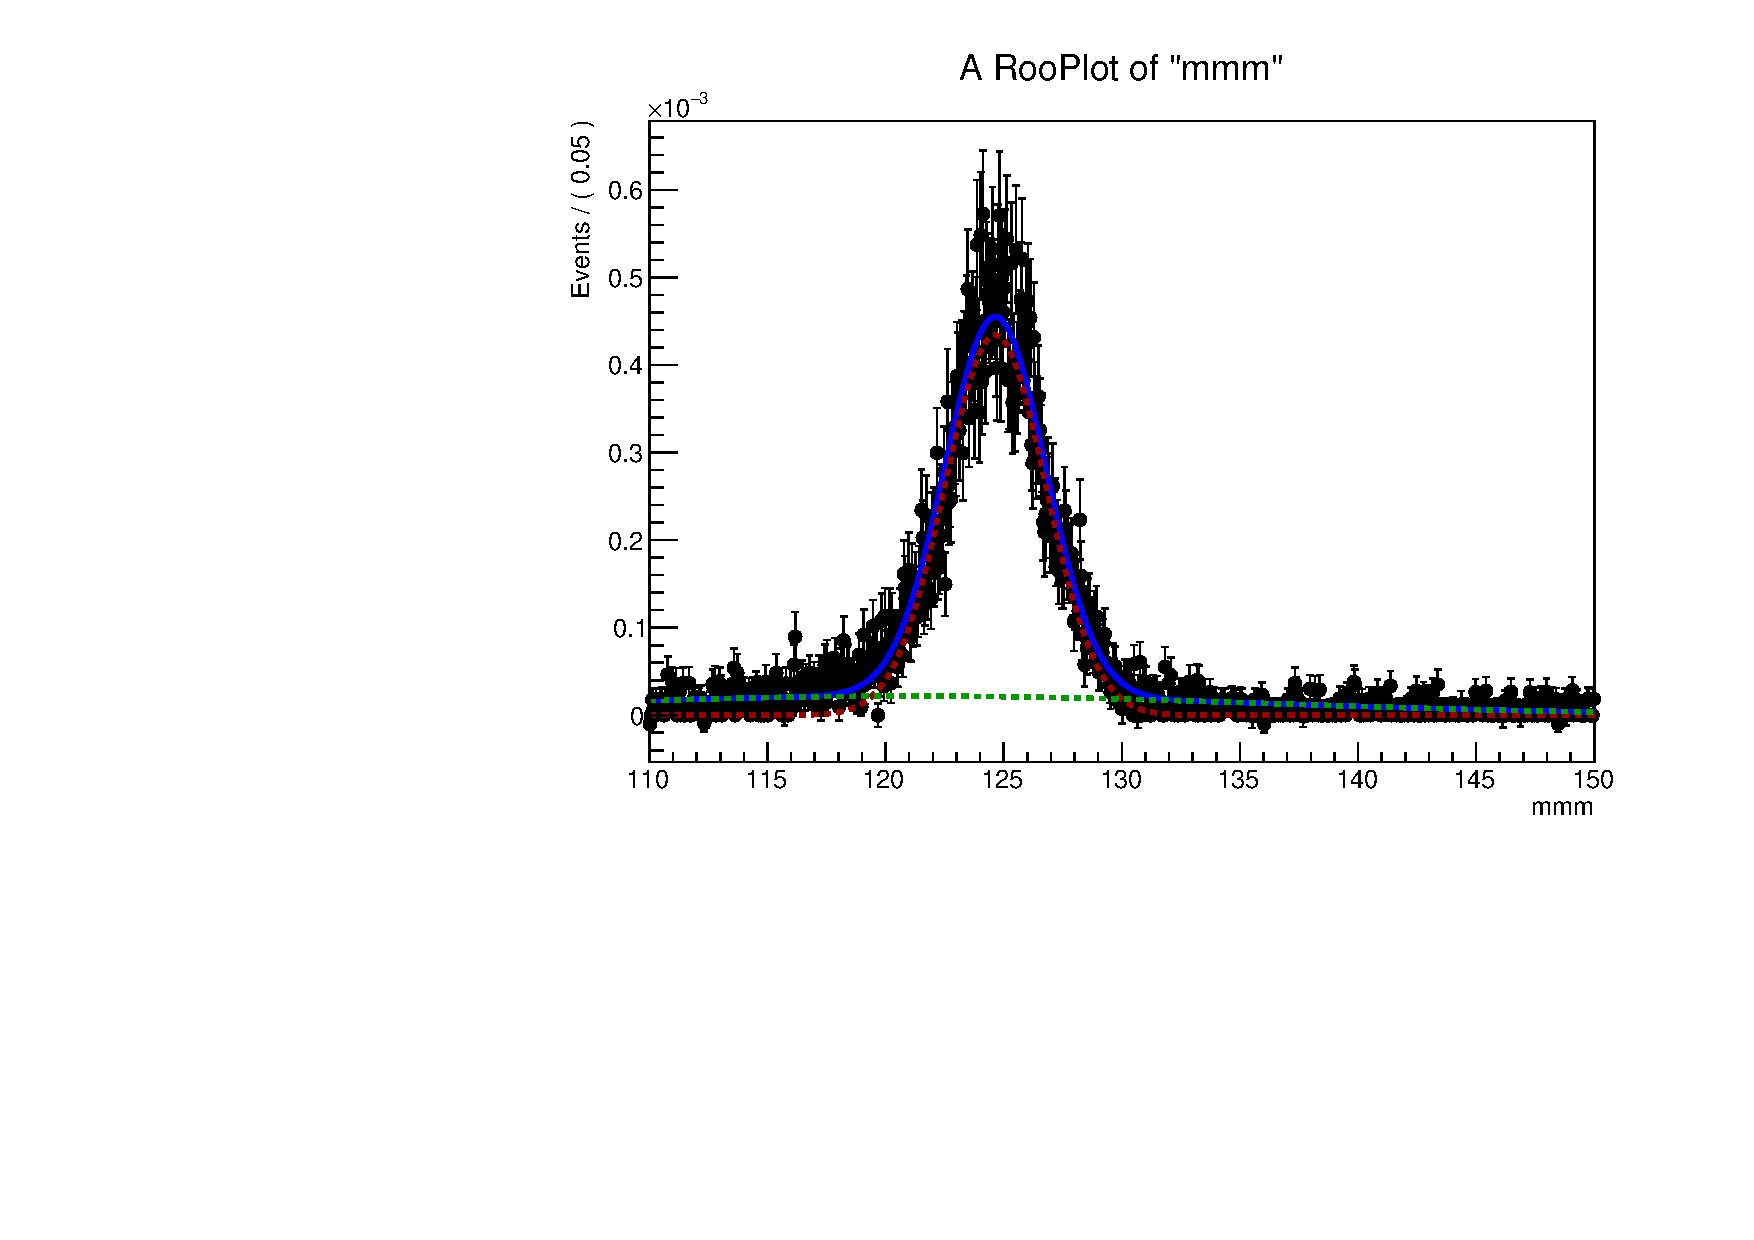
\includegraphics[width=.47\textwidth]{figures/signal_model/AppendixBdt/ttH/125/fit_mh_125_ttH_cat15.pdf}
}
 \\
\hline
\end{longtable}
